%@TheDoctorRAB
%standard white paper/preproposal format
%
%%%%%
%
%REFERENCES
%
%neup.bst - numbered citations in order of appearance, short author list with et al in reference section
%nsf.bst - numbered citations in order of appearance, full author list in references section
%standard.bst - citations with author last name with et al for more than 2 authors; full author list in references section
%ans.bst is for ANS only. 
%
%author = {Lastname, Firstname and Lastname, Firstname and Lastname, Firstname} for all bst formats
%bst renders the author list itself
%
%author = {{Nuclear Regulatory Commission}} if the author is an organization, institution, etc., and not people
%
%title = {{}} for all
%
%for all - use \citep{-} - [1] or (Borrelli, 2021) in the text
%standard.bst \cite{-} - Borrelli (2021) in the text
%standard.bst lists references alphabetically
%the rest list numerically
%
%
%%% slides 
%
%\citep{xxxnna} where the citation should go
%\blfootnote{\fontsize\cite{xxxnna}\fontsize\bibentry{xxxnna}} before \end{frame}
%
%
%%%%%

%%%%% presentation settings
\documentclass[aspectratio=1610,pdftex,dvipsnames,compress,xcolor={dvipsnames}]{beamer}
\usetheme{Boadilla}
\usecolortheme{seahorse}
\beamertemplatenavigationsymbolsempty
\addtobeamertemplate{footnote}{\hskip -2em}{} %pushes footnote to margin
\setbeamerfont{title}{series=\bfseries}
\setbeamertemplate{page number in head/foot}[framenumber] %just gives slide number; comment out for 1/7, 2/7...
\definecolor{BackGround}{RGB}{255,250,240}
\setbeamercolor{background canvas}{bg=BackGround}
%%%%%


%%%%% general 
%\documentclass[11pt,a4paper]{article}
%\usepackage[lmargin=1in,rmargin=1in,tmargin=1in,bmargin=1in]{geometry}
\usepackage[pagewise]{lineno} %line numbering
\usepackage{setspace}
\usepackage{ulem} %strikethrough - do not \sout{\cite{}}
\usepackage{graphicx}
\usepackage{mypythonhighlight,verbatim}
\usepackage{filecontents}
\usepackage{tablefootnote}
\usepackage{footnotehyper}
\usepackage{float}
%\usepackage{subfig}
\usepackage[yyyymmdd]{datetime} %date format
\renewcommand{\dateseparator}{.}
\graphicspath{{img/}} %path to graphics
\setcounter{secnumdepth}{5} %set subsection to nth level
\usepackage{needspace}
\usepackage[stable,hang,flushmargin]{footmisc} %footnotes in section titles and no indent; standard.bst
\usepackage[inline]{enumitem}
\setlist[itemize]{label=\textbullet}
\usepackage{boldline}
\usepackage{makecell}
\usepackage{booktabs}
\usepackage{amssymb}
\usepackage{gensymb}
\usepackage{amsmath,nicefrac}
\usepackage{physics}
\usepackage{lscape}
\usepackage{array}
\usepackage{chngcntr}
\usepackage{hyperref}
\hypersetup{colorlinks,linkcolor=black,citecolor=black,urlcolor=blue} 
%\usepackage{sectsty}
\usepackage{textcomp}
\usepackage{lastpage}
\usepackage{xargs} %for \newcommandx
\usepackage[colorinlistoftodos,prependcaption,textsize=tiny]{todonotes} %makes colored boxes for commenting
\usepackage{soul}
\usepackage{color}
\usepackage{marginnote}
\usepackage[figure,table]{totalcount}
\usepackage[capitalise]{cleveref}
\usepackage{microtype} %improves typography for pdf
\usepackage[pdftex,dvipsnames]{colortbl} %change font color
%%%%%


%%%%% tikz
\usepackage{pgf}
\usepackage{tikz} % required for drawing custom shapes
\usetikzlibrary{shapes,arrows,automata,trees}
%%%%%


%%%%% fonts
\usepackage{times}
%arial - uncomment next two lines
%\usepackage{helvet}
%\renewcommand{\familydefault}{\sfdefault}
%%%%%


%%%%% references
%\usepackage[round,semicolon]{natbib} %for (Borrelli 2021; Clooney 2019) - standard.bst 
\usepackage[numbers,sort&compress]{natbib} %for [1-3] - nsf.bst, neup.bst
\setlength{\bibsep}{7pt} %sets space between references
%\renewcommand{\bibsection}{} %suppresses large 'references' heading
%\renewcommand\bibpreamble{\vspace{\baselineskip}} %sets spacing after heading if not using default references heading
%%%%%


%%%%% tables and figures
\usepackage{longtable} %need to put label at top under caption then \\ - use spacing
\usepackage{tablefootnote}
\usepackage{tabularx}
\usepackage{multirow}
\usepackage{tabto} %general tabbed spacing
\usepackage{pdfpages}
\usepackage{wrapfig} %wraps figures around text
\setlength{\intextsep}{0.00mm}
\setlength{\columnsep}{1.00mm}
\usepackage[singlelinecheck=false,labelfont=bf]{caption}
\usepackage{subcaption}
\captionsetup[table]{justification=justified,skip=5pt,labelformat={default},labelsep=period,name={Table}} %sets a space after table caption
\captionsetup[figure]{justification=centering,skip=5pt,labelformat={default},labelsep=period,name={Figure}} %sets space above caption, 'figure' format
\captionsetup[wrapfigure]{justification=centering,aboveskip=0pt,belowskip=0pt,labelformat={default},labelsep=period,name={Fig.}} %sets space above caption, 'figure' format
\captionsetup[wraptable]{justification=centering,aboveskip=0pt,belowskip=0pt,labelformat={default},labelsep=period,name={Table}} %sets space above caption, 'figure' format
%%%%%


%%%%% watermark
%\usepackage[firstpage,vpos=0.63\paperheight]{draftwatermark}
%\SetWatermarkText{\shortstack{DRAFT\\do not distribute}}
%\SetWatermarkScale{0.20}
%%%%%


%%%%% cross referencing files
%\usepackage{xr} %for revisions - will cross reference from one file to here
%\externaldocument{/path/to/auxfilename} %aux file needed
%%%%%


%%%%% toc and glossaries
\usepackage[toc,title]{appendix}
\usepackage[acronym,nomain,nonumberlist]{glossaries}
\makenoidxglossaries
%\usepackage{titlesec,titletoc}
%\renewcommand{\thepart}{ARTICLE \Roman{part}} %puts the label into the command so \thelabel will carry through
%\renewcommand{\thesection}{\arabic{section}} %puts the label into the command so \thelabel will carry through
%\titleformat{\part}{\normalfont\large\bfseries}{\thepart}{}{}[]
%\titlespacing*\part{0pt}{0.95\baselineskip}{0.75\baselineskip}
%\titleformat{\section}[runin]{\normalfont\large\bfseries}{\thesection}{-1em}{}[.]
%\titlespacing*\section{0pt}{0.65\baselineskip}{0.55\baselineskip}
%\titleformat{\subsection}[runin]{\normalfont\normalsize\bfseries}{\thesubsection}{-1em}{}[.]
%\titlespacing*\subsection{0pt}{0.50\baselineskip}{0.35\baselineskip}
%\titleformat{\paragraph}[runin]{\normalfont\normalsize\bfseries\itshape}{\theparagraph}{-1em}{}[.]
%\titlespacing*\paragraph{0pt}{0.45\baselineskip}{0.25\baselineskip}
%\titleformat{\subparagraph}[runin]{\normalfont\normalsize\itshape}{\thesubparagraph}{-1em}{}[.]
%\titlespacing*\subparagraph{0pt}{0.40\baselineskip}{0.25\baselineskip}
%\titleformat{\paragraph}[hang]{\normalfont\normalsize\bfseries}{\theparagraph}{5pt}{}[]
%\titlespacing*\paragraph{0pt}{0.50\baselineskip}{0.25\baselineskip}
%\titleformat{\subparagraph}[runin]{\normalfont\normalsize\itshape}{\thesubparagraph}{-1em}{}[.]
%\titlespacing*\subparagraph{0pt}{0.40\baselineskip}{0.20\baselineskip}
%%%%%


%%%%% editing
\newcommand{\edit}[1]{\textcolor{blue}{#1}} %shortcut for changing font color on revised text
\newcommand{\fn}[1]{\footnote{#1}} %shortcut for footnote tag
\newcommand*\sq{\mathbin{\vcenter{\hbox{\rule{.3ex}{.3ex}}}}} %makes a small square as a separator $\sq$
%\newcommand{\sk}[1]{\sout{#1}} %shortcut for default strikethrough - do not sk through citep
\newcommand\sk{\bgroup\markoverwith{\textcolor{red}{\rule[0.5ex]{1pt}{1pt}}}\ULon} %strikethrough with red line; not in \section{}
%\st{} does strikethrough using soul package but does not like acronyms
%\newcommand{\blucell}{\cellcolor{aliceblue}} %use to shade in table cell
%\newcommand{\grycekk}{\cellcolor{lightgray}} %use to shade in table cell
%\newcommand{\whicell}{\cellcolor{antiquewhite}} %use to shade in table cell
%%%%%


%%%%% colors
%http://latexcolor.com/
%https://en.wikibooks.org/wiki/LaTeX/Colors#:~:text=black%2C%20blue%2C%20brown%2C%20cyan,be%20available%20on%20all%20systems.
\definecolor{aliceblue}{rgb}{0.94, 0.97, 1.0}
\definecolor{antiquewhite}{rgb}{0.98, 0.92, 0.84}
\definecolor{lightmauve}{rgb}{0.86, 0.82, 1.0}
\definecolor{brilliantlavender}{rgb}{0.96, 0.73, 1.0}
\definecolor{brandeisblue}{rgb}{0.0, 0.44, 1.0}
\definecolor{darkmidnightblue}{rgb}{0.0, 0.2, 0.4}

\newcommand{\x}{\cellcolor{aliceblue}} %use to shade in table cell
\newcommand{\y}{\cellcolor{lightgray}} %use to shade in table cell
\newcommand{\z}{\cellcolor{antiquewhite}} %use to shade in table cell
%%%%%


%%%%% acronyms
\newcommand{\acf}{\acrfull} %full acronym
\newcommand{\acl}{\acrlong} %long acronym
\newcommand{\acs}{\acrshort} %short acronym

\newcommand{\acfp}{\acrfullpl} %full acronym plural
\newcommand{\aclp}{\acrlongpl} %long acronym plural
\newcommand{\acsp}{\acrshortpl} %short acronym plural
%%%%%


%%%%% todonotes
\newcommandx{\cmt}[2][1=]{\todo[author=\textbf{STRUCTURE},tickmarkheight=0.15cm,linecolor=red,backgroundcolor=red!25,bordercolor=black,#1]{#2}}
\newcommandx{\con}[2][1=]{\todo[author=\textbf{CONTENT},tickmarkheight=0.15cm,linecolor=brilliantlavender,backgroundcolor=brilliantlavender,bordercolor=black,#1]{#2}}
\newcommandx{\rab}[2][1=]{\todo[noline,author=\textbf{RAB},backgroundcolor=Plum!25,bordercolor=black,#1]{#2}}


%\newcommandx{\jon}[2][1=]{\todo[noline,author=\textbf{ATTN: Johnson},backgroundcolor=blue!25,bordercolor=black,#1]{#2}}
%\newcommandx{\han}[2][1=]{\todo[noline,author=\textbf{ATTN: Haney},backgroundcolor=OliveGreen!25,bordercolor=black,#1]{#2}}
%\newcommandx{\rab}[2][1=]{\todo[author=\textbf{RAB},tickmarkheight=0.15cm,linecolor=Plum,backgroundcolor=Plum!25,bordercolor=black,#1]{#2}}
%\newcommandx{\han}[2][1=]{\todo[author=\textbf{ATTN: Haney},tickmarkheight=0.15cm,linecolor=OliveGreen,backgroundcolor=OliveGreen!25,bordercolor=OliveGreen,#1]{#2}}
%\newcommandx{\jon}[2][1=]{\todo[author=\textbf{ATTN: Johnson},tickmarkheight=0.15cm,linecolor=blue,backgroundcolor=blue!25,bordercolor=blue,#1]{#2}}


% highlighting 
\DeclareRobustCommand{\hlc}[1]{{\sethlcolor{LimeGreen}\hl{#1}}}
\makeatletter
    \if@todonotes@disabled
    \newcommand{\hlh}[2]{#1}
    \else
    \newcommand{\hlh}[2]{\han{#2}\hlc{#1}}
    \fi
    \makeatother

\DeclareRobustCommand{\hld}[1]{{\sethlcolor{CornflowerBlue}\hl{#1}}}
\makeatletter
    \if@todonotes@disabled
    \newcommand{\hlj}[2]{#1}
    \else
    \newcommand{\hlj}[2]{\jon{#2}\hld{#1}}
    \fi
    \makeatother

\DeclareRobustCommand{\hlf}[1]{{\sethlcolor{lightmauve}\hl{#1}}}
\makeatletter
    \if@todonotes@disabled
    \newcommand{\hlb}[2]{#1}
    \else
    \newcommand{\hlb}[2]{\rab{#2}\hlf{#1}}
    \fi
    \makeatother
%%%%%


%%%%% table alignments
\newcolumntype{L}[1]{>{\raggedright\let\newline\\\arraybackslash\hspace{0pt}}m{#1}} %uses \raggedright with m,p{} in table column
\newcolumntype{C}[1]{>{\centering\let\newline\\\arraybackslash\hspace{0pt}}m{#1}} %uses \raggedright with m,p{} in table column
\newcolumntype{R}[1]{>{\raggedleft\let\newline\\\arraybackslash\hspace{0pt}}m{#1}} %uses \raggedright with m,p{} in table column
%%%%%


%%%%% table contents
\makeatletter
\renewcommand\tableofcontents{%
    \@starttoc{toc}%
}
\makeatother

\makeatletter
\renewcommand\listoffigures{%
    \@starttoc{lof}%
}
\makeatother

\makeatletter
\renewcommand\listoftables{%
    \@starttoc{lot}%
}
\makeatother

\makeatletter
\newcommand*\ftp{\fontsize{16.5}{17.5}\selectfont}
\makeatother
%%%%%


%%%%% user commands
\newcommand\blfootnote[1]{%
  \begingroup
  \renewcommand\thefootnote{}\footnote{#1}%
  \addtocounter{footnote}{-1}%
  \endgroup
}

\makeatletter
\renewcommand{\@biblabel}[1]{#1.\hfill} %bibliography ordered list has numbers left flush
\makeatother
%%%%%

%%%%% archived section commands - use titlesec
%\makeatletter
%\renewcommand\section{%
%    \@startsection{section}{1}{\z@ }{0.50\baselineskip}{0.25\baselineskip}
%    {\large \normalfont \bfseries}}%

%\makeatletter
%\renewcommand\paragraph{%
%    \@startsection{paragraph}{4}{\z@ }{0.55\baselineskip}{-1em}
%    {\normalfont \normalsize \bfseries}}%

%\makeatletter
%\renewcommand\subparagraph{%
%    \@startsection{subparagraph}{5}{\z@ }{0.40\baselineskip}{-1em}
%    {\normalfont \normalsize \itshape }}%

%\makeatletter
%\renewcommand\subsection{%
%    \@startsection{subsection}{2}{\z@ }{0.45\baselineskip}{0.25\baselineskip}
%    {\large \normalfont \bfseries}}%
%%%%%


%%%%% header and footer
%\usepackage{fancyhdr}
%\pagestyle{fancy}
%\fancyhf{} %move page number to bottom right
%\renewcommand{\headrulewidth}{0pt} %set line thickness in header; uncomment as is to remove line
%\lhead{\scriptsize Name}
%\lhead{\scriptsize PNUCENE-D-22-xxxxx}
%\chead{\scriptsize \textit{PhD White Paper Project Proposal}}
%\rhead{\scriptsize \today}
%\rfoot{\thepage}
%%%%%


%%%%%%% citations
%\begin{filecontents}{references.bib}
%\end{filecontents}
%%%%%%%


%%%%% acronyms
% alphabetical ordering is automated
\newacronym{nrs}{NRHES}{Nuclear Renewable Hybrid Energy System}
\newacronym{ahp}{AHP}{Analytical Hierarchy Process}
\newacronym{inl}{INL}{Idaho National Laboratory}
\newacronym{orl}{ORNL}{Oak Ridge National Laboratory}
\newacronym{anl}{ANL}{Argonne National Laboratory}
\newacronym{npp}{NPP}{Nuclear Power Plant}
\newacronym{smr}{SMR}{Small Modular Reactor}
\newacronym{ump}{UAMPS}{Utah Associated Municipal Power Systems}
\newacronym{nus}{NuScale}{NuScale Power, LLC}
\newacronym{nrc}{NRC}{United States Nuclear Regulatory Commission}
\newacronym{epri}{EPRI}{Electric Power Research Institute}
\newacronym{nerc}{NERC}{North American Electric Reliability Corporation}
\newacronym{ci}{CI}{Consistency Index}
\newacronym{cr}{CR}{Consistency Ratio}
\newacronym{htse}{HTSE}{High Temperature Steam Electrolysis}
\newacronym{lwr}{LWR}{Light Water Reactor}
\newacronym{eia}{EIA}{U.S. Energy Information Administration}
\newacronym{oer}{OER}{Online Educational Resource}
\newacronym{lms}{LMS}{Learning Management System}
\newacronym{cps}{CPS}{Cyber-Physical Systems}
\newacronym{nsf}{NSF}{National Science Foundation}
\newacronym{wsc}{WSC}{Western Services Corporation}
\newacronym{cae}{CAES}{Center for Advanced Energy Studies}
\newacronym{hsl}{HSSL}{Human System Simulation Laboratory}
\newacronym{pwr}{PWR}{Pressurized Water Reactor}
\newacronym{bwr}{BWR}{Boiling Water Reactor}
\newacronym{roi}{ROI}{Return on Investment}
\newacronym{ic}{I\&C}{Instrumentation \& Controls}
\newacronym{mwe}{MWe}{Megawatts-electric}
\newacronym{ics}{ICS}{Industrial Control Systems}
\newacronym{sca}{SCADA}{Supervisory Control and Data Acquisition}
\newacronym{ip}{IP}{Internet Protocol}
\newacronym{udp}{UDP}{User Datagram Protocol}
\newacronym{tva}{TVA}{Tennessee Valley Authority}
\newacronym{plc}{PLC}{Programmable Logic Controller}
\newacronym{vfd}{VFD}{Variable Frequency Drive}
\newacronym{khp}{KHNP}{Korean Hydro \& Nuclear Power Co., Ltd}
\newacronym{onl}{ORNL}{Oak Ridge National Laboratory}
\newacronym{jcp}{JCPOA}{Joint Comprehensive Plan of Action}
\newacronym{mim}{MITM}{Man in the Middle}
\newacronym{dos}{DDoS}{Distributed Denial of Service}
\newacronym{tcp}{TCP/IP}{Transmission Control Protocol/Internet Protocol}
\newacronym{dnp}{DNP3}{Distributed Network Protocol 3}
\newacronym{pra}{PRA}{Probabilistic Risk Assessment}
\newacronym{cs}{CS}{Critical System}
\newacronym{loc}{LOCA}{Loss of Coolant Accident}
\newacronym{hmi}{HMI}{Human Machine Interface}
\newacronym{pha}{PHA}{Preliminary Hazards Analysis}
\newacronym{bol}{BOL}{Beginning-of-Life}
\newacronym{eol}{EOL}{End-of-Life}
\newacronym{mol}{MOL}{Middle-of-Life}
\newacronym{imu}{IMUNES}{Integrated Multiprotocol Network Emulator/Simulator}
\newacronym{ccc}{CCC}{Computing Community Consortium}
\newacronym{neu}{NEUP}{Nuclear Energy University Program}
\newacronym{doe}{DOE}{United States Department of Energy}
\newacronym{nei}{NEI}{Nuclear Energy Institute}
\newacronym{nit}{NITRD}{Networking Information Technology Research \& Development Program}
\newacronym{rcs}{RCS}{Reactor Cooling System}
\newacronym{con}{IC}{Initial Condition}
\newacronym{csi}{CSIS}{Center for Strategic \& International Studies}
\newacronym{pcap}{PCAP}{packet capture file}
\newacronym{dc}{DC}{Direct-Current}
\newacronym{ac}{AC}{Alternating-Current}
\newacronym{iff}{UIIF}{Idaho Falls Center for Higher Education}
\newacronym{snl}{SNL}{Sandia National Laboratory}
\newacronym{cie}{CIE}{Cyber-Informed Engineering}
\newacronym{cds}{CRDS}{Control Rod Drive System}
\newacronym{cdm}{CRDM}{Control Rod Drive Mechanism}
\newacronym{fma}{FMEA}{Failure Modes \& Effects Analysis}
\newacronym{rpn}{RPN}{Risk Priority Number}
\newacronym{scr}{SCR}{silicon controller rectifier}
\newacronym{hvc}{HVAC}{Heating, Ventilation \& Air Conditioning}
\newacronym{ttb}{TTB}{Time-to-Boil}
\newacronym{sis}{SIS}{Safety Instrumented System}
\newacronym{ui}{UI}{University of Idaho}
\newacronym{swu}{SWU}{Separative Work Unit}
\newacronym{cp1}{CP-1}{Chicago Pile-1}
\newacronym{eb1}{EBR-I}{Experimental Breeder Reactor-I}
\newacronym{eb2}{EBR-II}{Experimental Breeder Reactor-II}
\newacronym{trt}{TREAT}{Transient Reactor Test Facility}
\newacronym{cdu}{CANDU}{Canada Deuterium Uranium}
\newacronym{wip}{WIPP}{Waste Isolation Pilot Plant}
\newacronym{tpa}{TSPA}{Total System Performance Assessment}
\newacronym{nwa}{NWPA}{Nuclear Waste Policy Act}
\newacronym{brc}{BRC}{Blue Ribbon Commission}
\newacronym{pur}{PUREX}{Plutonium Uranium Reduction Extraction}
\newacronym{mox}{MOX}{Mixed Oxide}
\newacronym{tbp}{TBP}{tributyl phosphate}
\newacronym{fp}{FP}{fission product}
\newacronym{nas}{NAS}{National Academy of Sciences}
\newacronym{tru}{TRU}{Transuranic Elements}
\newacronym{hlw}{HLW}{High Level Waste}
\newacronym{sfr}{SFR}{Sodium Fast Reactor}
%\newacronym{}{}{}
%%%%%


%%%%% spacing
%\onehalfspacing %linespacing
%\setstretch{1.05} %linespacing
%\spacing{1.25} %equivalent to 1.5 line spacing in Word
%%%%%


%%%%% linenumbering
%\linenumbers %toggle line numbers
%\pagewiselinenumbers %reset line numbers on new page
%\modulolinenumbers[1] %line numbering interval
%%%%%


%%%%% title page
\addtocounter{framenumber}{-1} %does not count the title slide in the slide count
\title[NE585 - Nuclear fuel cycles]{NE585\\NUCLEAR FUEL CYCLES\\Front end of the nuclear fuel cycle\\3}
\author[@TheDoctorRAB]{R. A. Borrelli}
\institute[]{
    \acl{ui}\\
    \vspace{0.10in}
    
\includegraphics[width=0.20\textwidth]{ne-logo.png}
    }
\date{\acl{iff}}
%%%%%


\begin{document}


%%%%% title page with no footer
{
    \setbeamertemplate{footline}{}
    \begin{frame}
        \titlepage
    \end{frame}
}
%%%%%


\begin{frame}{Learning objectives}
    \begin{enumerate}[series=outerlist,topsep=0pt,itemsep=15pt,leftmargin=*,label=(\arabic*)]
        \item[]Demonstrating how the nuclear fuel cycle is an holistic system
        \item[]Explaining why the nuclear fuel cycle is what it is
        \item[]Apply principle of \acs{swu}
        \item[]Model a nominal solvent extraction system
        \item[]Model enrichment processes
        \item[]Demonstrate principles of enrichment and converstion
        \item[]Some of Chapter 4 in the book
        \item[]Check out \href{http://pandoraspromise.com/}{Pandora's promise} if it's still on Netflix
        \item[]There's a lot of pictures here
    \end{enumerate}
\end{frame}


\begin{frame}{Learning nodes}
    \begin{columns}[t]

        \begin{column}{0.50\textwidth}
            \begin{enumerate}[series=outerlist,topsep=0pt,itemsep=1pt,leftmargin=*,label=(\arabic*)]
                \item[]\textbf{Nuclear fuel cycle overview}
                    \vspace{0.15in}
                \item[]\textbf{Locations of current domestic fleet}
                    \vspace{0.15in}
                \item[]\textbf{Plant closures}
                    \vspace{0.15in}
                \item[]\textbf{Nuclear power around the world}
                    \vspace{0.15in}
                \item[]\textbf{Planned construction}
                    \vspace{0.15in}
                \item[]\textbf{Components of the nuclear fuel cycle}
                \item[]Mining
                \item[]Milling
                \item[]Conversion
                \item[]Enrichment
                \item[]\acf{swu}
                \item[]Fuel fabrication
            \end{enumerate}
        \end{column}

        \begin{column}{0.50\textwidth}
            \begin{enumerate}[series=outerlist,topsep=0pt,itemsep=1pt,leftmargin=*,label=(\arabic*)]
                \item[]\hfill\textbf{Macro reactor operation}
                \item[]\hfill \acs{cp1}
                \item[]\hfill Hanford B reactor
                \item[]\hfill \acs{eb1}
                \item[]\hfill \acs{eb2}
                \item[]\hfill \acs{trt} 
                \item[]\hfill Military use
                    \vspace{0.15in}
                \item[]\hfill\textbf{Reactor concepts}
                \item[]\hfill Generations
                \item[]\hfill \acs{pwr}
                \item[]\hfill \acs{bwr}
                \item[]\hfill \acs{cdu}
                    \vspace{0.15in}
                \item[]\hfill\textbf{Aqueous reprocessing}
            \end{enumerate}
        \end{column}

    \end{columns}
\end{frame}


\begin{frame}{More learning nodes}
    \begin{enumerate}[series=outerlist,topsep=0pt,itemsep=1pt,leftmargin=*,label=(\arabic*)]
        \item[]\textbf{Enrichment}
        \item[]History
        \item[]Processing
        \item[]Tails
            \vspace{0.15in}
        \item[]\textbf{Conversion}
        \item[]Processing
    \end{enumerate}
\end{frame}


\begin{frame}[plain]{}
    \centering\LARGE\textbf{Nuclear fuel cycle overview}
\end{frame}


\addtocounter{framenumber}{-1} 
\begin{frame}{}
    \begin{figure}
        \centering
        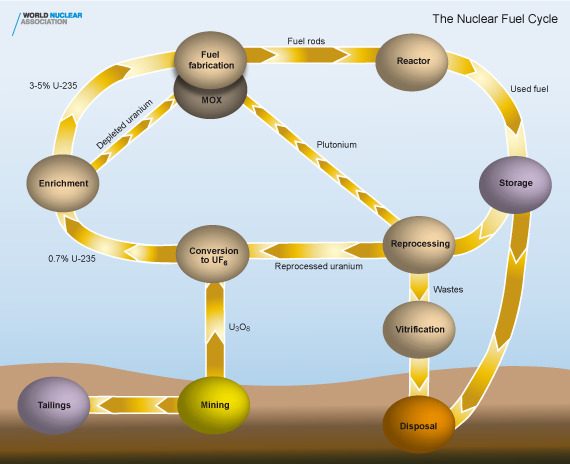
\includegraphics[width=0.75\textwidth]{nuclear.fuel.cycle1.jpg}
%        \caption{}
    \end{figure}
\end{frame}


\begin{frame}{}
    \begin{figure}
        \centering
        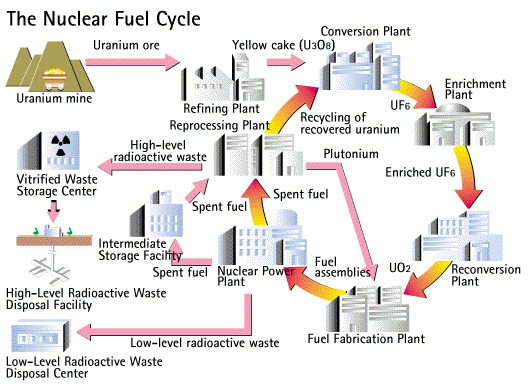
\includegraphics[width=0.75\textwidth]{nuclear.fuel.cycle2.jpg}
%        \caption{}
    \end{figure}
\end{frame}

\begin{frame}{}
    \begin{figure}
        \centering
        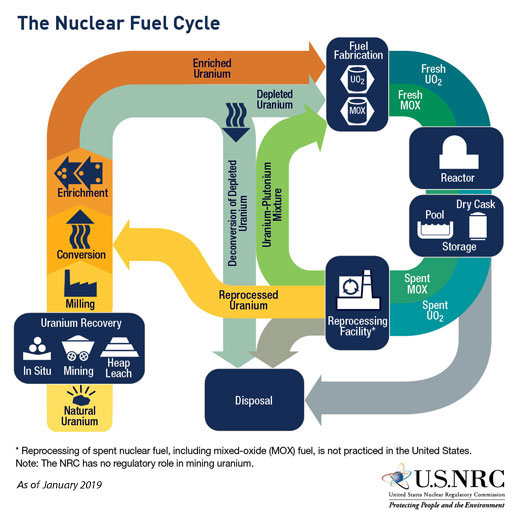
\includegraphics[width=0.65\textwidth]{nuclear.fuel.cycle3.jpg}
%        \caption{}
    \end{figure}
\end{frame}


\begin{frame}{Look at the fuel cycle as systems engineering}
    \begin{enumerate}[series=outerlist,topsep=0pt,itemsep=21pt,leftmargin=*,label=(\arabic*)]
        \item[]Mining
        \item[]Making the fuel (saw Areva plant in Richland)
        \item[]What a reactor does and the different kinds
        \item[]Recycling (what kinds and how)
        \item[]Back-end management (storage and disposal)
        \item[]The fuel cycle has a lot of technical but institutional issues too
        \item[]How are they functionally dependent? 
    \end{enumerate}
\end{frame}


\begin{frame}{The fuel used in the commercial reactors is $UO_2$ or $ (Pu+U)O_2$}
    \begin{columns}[t]

        \begin{column}{0.55\textwidth}
            \begin{figure}
                \centering
                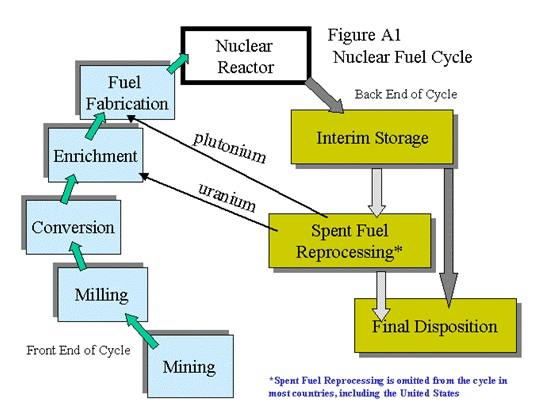
\includegraphics[width=0.95\textwidth]{cycle.components.jpg}
                %\caption{}
            \end{figure}
        \end{column}

        \begin{column}{0.45\textwidth}
            \begin{enumerate}[series=outerlist,topsep=0pt,itemsep=21pt,leftmargin=*,label=(\arabic*)]
                \item[]\textbf{Front end} -- Making the fuel and putting it in the reactor
                \item[]\textbf{Back end} -- What happens when you take it out of the reactor
            \end{enumerate}
        \end{column}

    \end{columns}
\end{frame}


\begin{frame}[plain]{}
    \centering\LARGE\textbf{Locations of current domestic fleet}
\end{frame}


\addtocounter{framenumber}{-1} 
\begin{frame}{}
    \begin{figure}
        \centering
        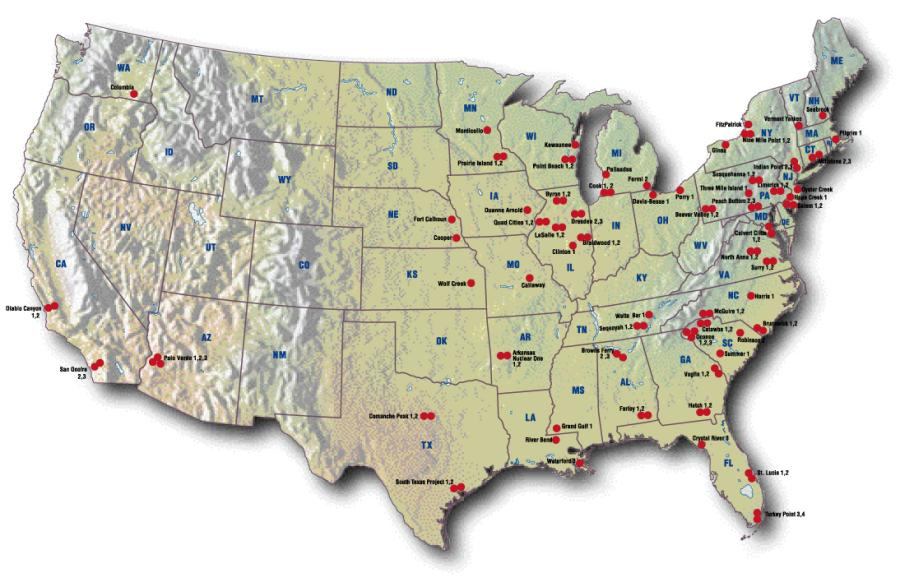
\includegraphics[width=0.95\textwidth]{nuclear.reactor.sites.jpg}
%        \caption{}
    \end{figure}
\end{frame}


\begin{frame}{}
    \begin{figure}
        \centering
        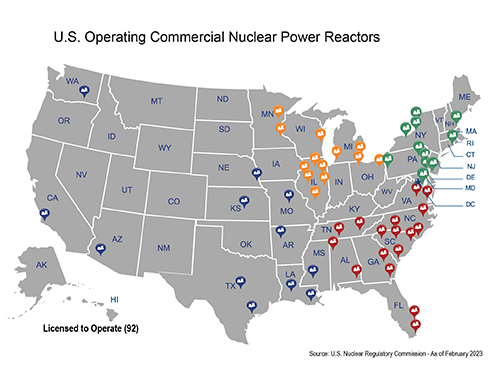
\includegraphics[width=0.85\textwidth]{power-reactors-operating.png}
%        \caption{}
    \end{figure}
\end{frame}


\begin{frame}[plain]{}
    \centering\LARGE\textbf{\href{https://www.nrc.gov/reactors/operating/list-power-reactor-units.html}{\acs{nrc} list of power reactor units}}
\end{frame}


\addtocounter{framenumber}{-1} 
\begin{frame}{}
    \begin{figure}
        \centering
        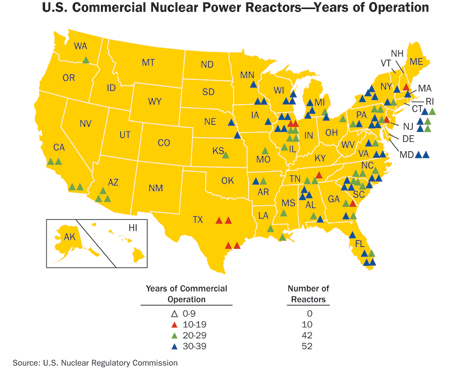
\includegraphics[width=0.75\textwidth]{plant.life.cycle.jpg}
%        \caption{}
    \end{figure}
\end{frame}


\begin{frame}[plain]{}
    \centering\LARGE\textbf{\href{https://uidaho.pressbooks.pub/nuclearengineering/chapter/fuel-cycle-overview/}{Plant closures}}
\end{frame}


\addtocounter{framenumber}{-1} 
\begin{frame}{}
    \begin{figure}
        \centering
        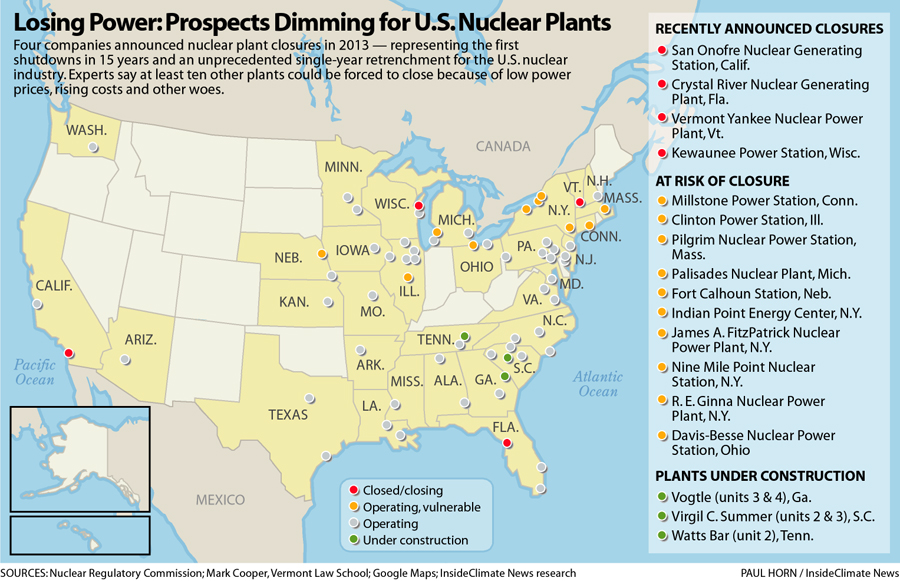
\includegraphics[width=0.75\textwidth]{plant.closures.jpg}
%        \caption{}
    \end{figure}
\end{frame}


\begin{frame}[plain]{}
    \centering\LARGE\textbf{Let's look at other nations}
\end{frame}


\addtocounter{framenumber}{-1} 
\begin{frame}{}
    \begin{figure}
        \centering
        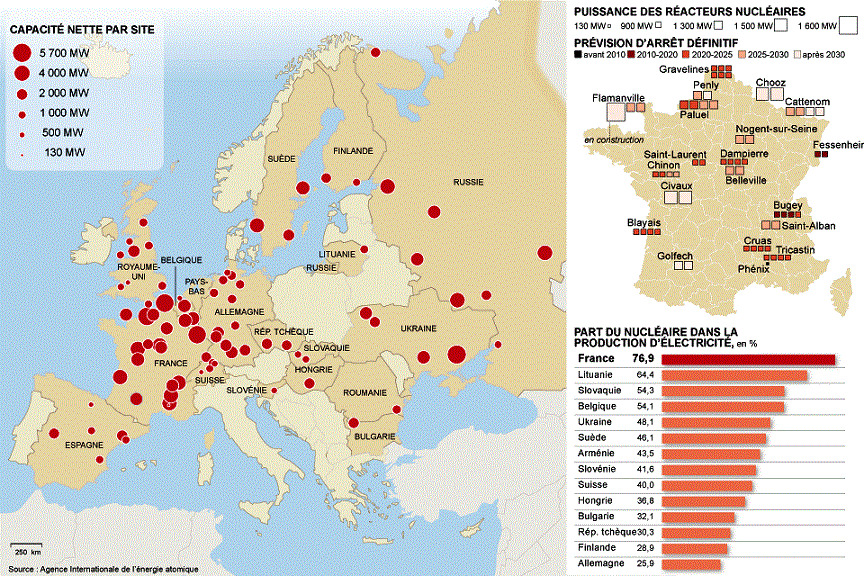
\includegraphics[width=0.75\textwidth]{europe.jpg}
%        \caption{}
    \end{figure}
\end{frame}


\begin{frame}{}
    \begin{figure}
        \centering
        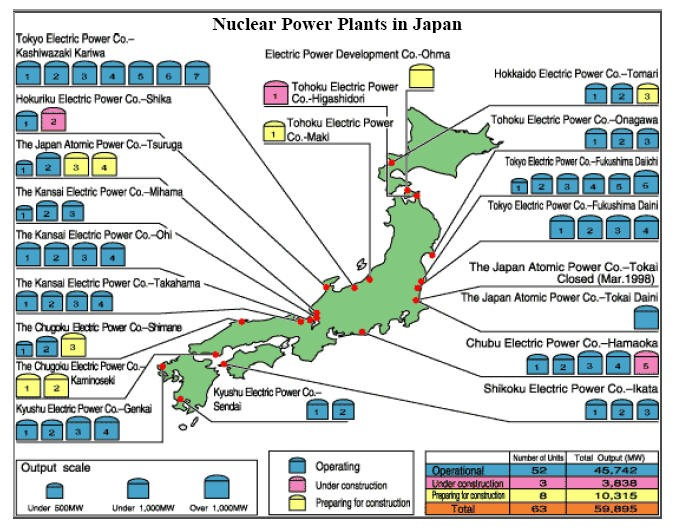
\includegraphics[width=0.75\textwidth]{japan.jpg}
%        \caption{}
    \end{figure}
\end{frame}


\begin{frame}{Where are they going to dispose of everything?}
    \begin{figure}
        \centering
        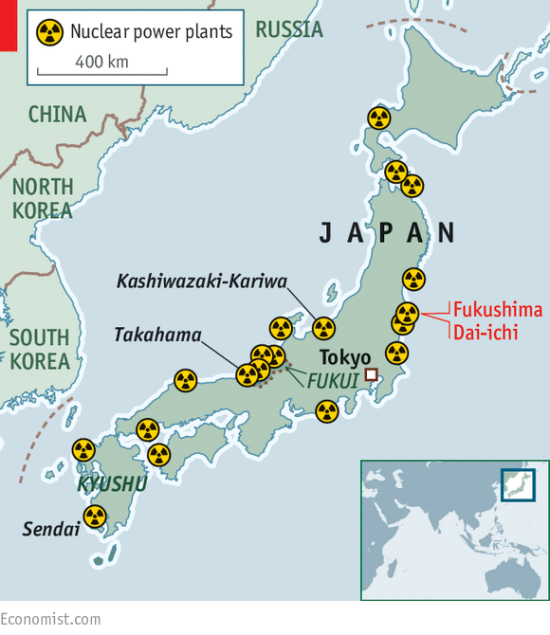
\includegraphics[width=0.45\textwidth]{japan2.jpg}
%        \caption{}
    \end{figure}
\end{frame}


\begin{frame}{Same problem}
    \begin{figure}
        \centering
        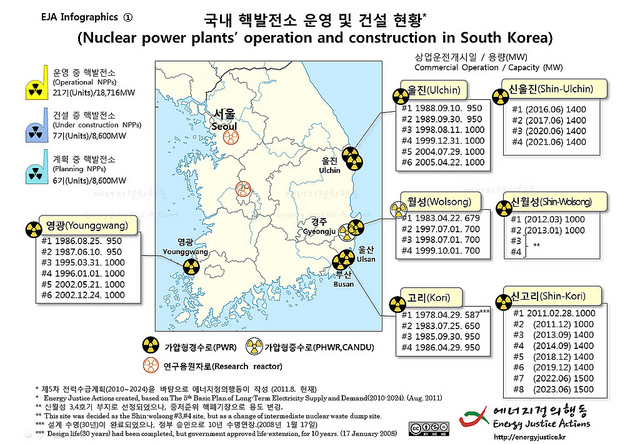
\includegraphics[width=0.75\textwidth]{korea.jpg}
%        \caption{}
    \end{figure}
\end{frame}


\begin{frame}{}
    \begin{figure}
        \centering
        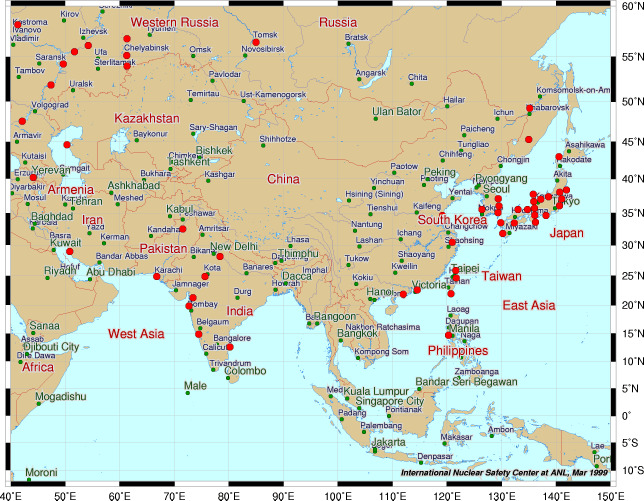
\includegraphics[width=0.75\textwidth]{asia.jpg}
%        \caption{}
    \end{figure}
\end{frame}


\begin{frame}[plain]{}
    \centering\LARGE\textbf{\href{https://www.world-nuclear.org/information-library/current-and-future-generation/plans-for-new-reactors-worldwide.aspx}{Planned construction}}
\end{frame}


\begin{frame}[plain]{}
    \centering\LARGE\textbf{Components of the nuclear fuel cycle}
\end{frame}


\begin{frame}[plain]{}
    \centering\LARGE\textbf{Mining}
\end{frame}


\addtocounter{framenumber}{-3} 
\begin{frame}{We have to find uranium first \href{https://www.uxc.com/p/prices/UxCPrices.aspx}{$U_3O_8$}}
    \begin{columns}[c]

        \begin{column}{0.55\textwidth}
            \begin{figure}
                \centering
                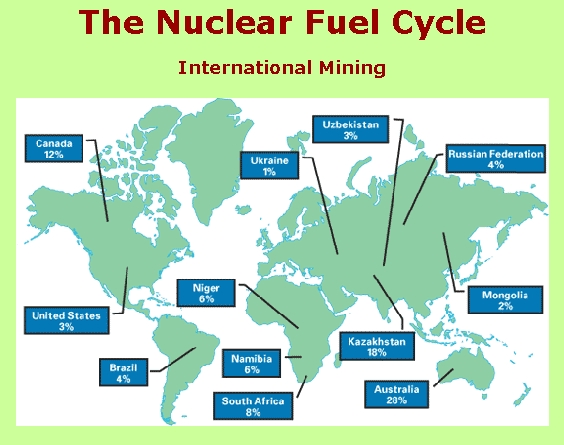
\includegraphics[width=0.95\textwidth]{uranium.world.jpg}
                %\caption{}
            \end{figure}
        \end{column}

        \begin{column}{0.45\textwidth}
            \begin{enumerate}[series=outerlist,topsep=0pt,itemsep=21pt,leftmargin=*,label=(\arabic*)]
                \item[]Extract the ore from the ground
                \item[]What do you do if you don't have it?
                \item[]Check out Australia
            \end{enumerate}
        \end{column}

    \end{columns}
\end{frame}


\begin{frame}[plain]{}
    \centering\LARGE\textbf{Milling}
\end{frame}


\addtocounter{framenumber}{-1} 
\begin{frame}{Uranium ore is refined by milling}
    \begin{enumerate}[series=outerlist,topsep=0pt,itemsep=18pt,leftmargin=*,label=(\arabic*)]
        \item[]The ore contains $UO_2, \; UO_3$ and other heavy metal oxides
        \item[]Usually using solvents to leach it from the ground
        \item[]Then it is chemically treated to obtain \href{http://ibankcoin.com/zeropointnow/files/2017/11/c5fbed2f-575a-41bb-886e-f26700d43255-2060x1236-2.jpeg}{`yellowcake'}
        \item[]Lots of contaminated scrap is produced though (mill tailings)
        \item[]Usually dumped as sludge in ponds (lots)
        \item[]Radioisotopes (radon), heavy metals, chemicals, etc.
        \item[]We have plenty of uranium resources
        \item[]But what if we decide it is too harmful to mine?
    \end{enumerate}
\end{frame}


\begin{frame}[plain]{}
    \centering\LARGE\textbf{Conversion}
\end{frame}


\addtocounter{framenumber}{-1} 
\begin{frame}{$U_3O_8$ is converted to $UF_6$ prior to enrichment}
    \begin{enumerate}[series=outerlist,topsep=0pt,itemsep=21pt,leftmargin=*,label=(\arabic*)]
        \item[]Mined U contains $^{234}U$, $^{235}U$, $^{238}U$, .0054\%, .72\%
        \item[]Because it is a gas at not so high temperature which is easier for enrichment
    \end{enumerate}
\end{frame}


\begin{frame}[plain]{}
    \centering\LARGE\textbf{Enrichment}
\end{frame}


\addtocounter{framenumber}{-1} 
\begin{frame}{$UF_6$ gas is then enriched with $^{235}U$}
    \begin{enumerate}[series=outerlist,topsep=0pt,itemsep=21pt,leftmargin=*,label=(\arabic*)]
        \item[]Enriched to 3\% to 5\%
        \item[]The byproduct is depleted uranium DU
        \item[]Used for armor and bullets
        \item[]Any idea why?
    \end{enumerate}
\end{frame}


\begin{frame}{}
    \begin{figure}
        \centering
        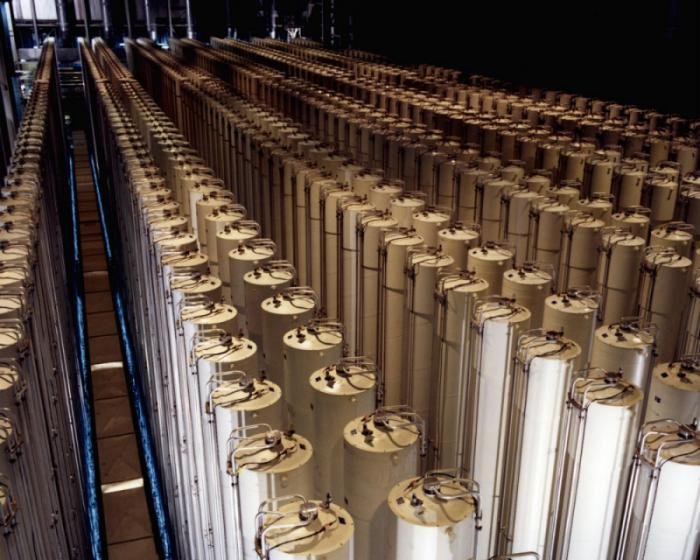
\includegraphics[width=0.75\textwidth]{centrifuges.jpg}
%        \caption{}
    \end{figure}
\end{frame}


\begin{frame}{}
    \begin{figure}
        \centering
        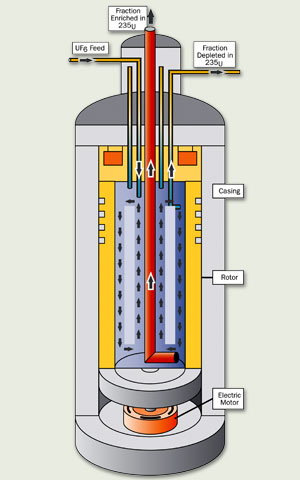
\includegraphics[width=0.35\textwidth]{centrifuge.jpg}
%        \caption{}
    \end{figure}
\end{frame}


\begin{frame}[plain]{}
    \centering\LARGE\textbf{\acf{swu}}
\end{frame}


\addtocounter{framenumber}{-1} 
\begin{frame}{\acs{swu} is the \href{https://uidaho.pressbooks.pub/nuclearengineering/chapter/swu/}{amount of work} to enrich uranium from natural abundance to reactor/weapon grade}
    \begin{enumerate}[series=outerlist,topsep=0pt,itemsep=21pt,leftmargin=*,label=(\arabic*)]
        \item[]Dumb acronyms are why people hate nuclear
    \end{enumerate}

    \vspace*{\fill}

    \begin{equation}
        \LARGE
        x_F = 0.0072
    \end{equation}

    \begin{equation}
        \LARGE 
        x_P = 0.03 - 0.05
    \end{equation}

    \begin{equation}
        \LARGE 
        x_W = 0.0002 - 0.0003
    \end{equation}
    
    \vspace*{\fill}

    \begin{enumerate}[series=outerlist,topsep=0pt,itemsep=21pt,leftmargin=*,label=(\arabic*)]
        \item[]Amount of feed for target product increases linearly with $x_P$ by mass conservation
    \end{enumerate}
\end{frame}


\begin{frame}{}
    \begin{columns}[c]

        \begin{column}{0.55\textwidth}
            \begin{figure}
                \centering
                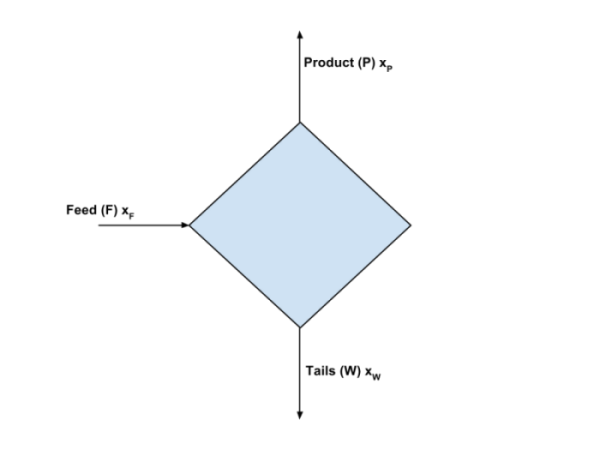
\includegraphics[width=0.95\textwidth]{mass.conservation.jpg}
                %\caption{}
            \end{figure}
        \end{column}

        \begin{column}{0.45\textwidth}
            \begin{equation}
                \LARGE 
                F = P + W
            \end{equation}

            \begin{equation}
                \LARGE 
                F \cdot x_F = P \cdot x_P + W \cdot x_W
            \end{equation}
        \end{column}

    \end{columns}
\end{frame}


\begin{frame}{\acs{swu} measures thermodynamic work to separate isotopes}
    \begin{enumerate}[series=outerlist,topsep=0pt,itemsep=11pt,leftmargin=*,label=(\arabic*)]
        \item[]\acs{swu} has units of kg because of course it does
        \item[]Separation potential is a measure of differences in Gibbs free energy
    \end{enumerate}

    \vspace*{\fill}

    \begin{equation}
        \LARGE
        SWU \equiv [P \cdot V(x_P)+W \cdot V(x_W)]-F \cdot V(x_F)
    \end{equation}

    \begin{equation}
        \LARGE 
        V(x_i) \equiv (2x_i - 1) \cdot ln \frac{x_i}{1-x_i}
    \end{equation}
    
    \begin{equation}
        \LARGE 
        \frac{SWU}{P} = V(x_P) + \frac{W}{P}V(x_W) - \frac{F}{P}V(x_F)
    \end{equation}
    
    \vspace*{\fill}

    \begin{enumerate}[series=outerlist,topsep=0pt,itemsep=11pt,leftmargin=*,label=(\arabic*)]
        \item[]The derivation is based on entropy changes
        \item[]Change in entropy in \href{https://drive.google.com/file/d/0B1ENwqH9aCq5UnZ4NHNCdHZfN1U/view?resourcekey=0-WXKzU2rJK0q2qVPJcDhutQ}{binary mixture of gases}
    \end{enumerate}
\end{frame}


\begin{frame}{}
    \begin{figure}
        \centering
        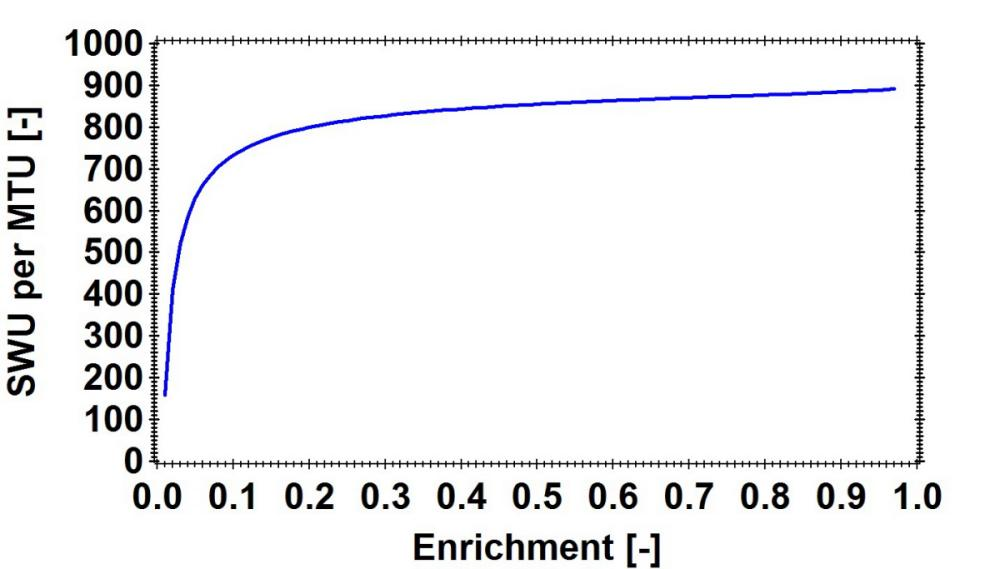
\includegraphics[width=0.95\textwidth]{swu.jpg}
%        \caption{}
    \end{figure}
\end{frame}


\begin{frame}[plain]{}
    \centering\LARGE\textbf{Fuel Fabrication}
\end{frame}


\addtocounter{framenumber}{-1} 
\begin{frame}{The fuel fabrication process (\acsp{lwr}) makes ceramic $UO_2$ pellets}
    \begin{enumerate}[series=outerlist,topsep=0pt,itemsep=21pt,leftmargin=*,label=(\arabic*)]
        \item[]Why ceramic?
        \item[]Is there anything better?
        \item[]Fuel rods contain a Zr-based alloy
        \item[]\href{https://inis.iaea.org/collection/NCLCollectionStore/_Public/47/032/47032411.pdf}{Also generates hydrogen gas}
    \end{enumerate}

    \vspace*{\fill}

    \begin{equation}
        \LARGE 
        Zr+2H_2O \rightarrow ZrO_2+2H_2
    \end{equation}
    
    \vspace*{\fill}

    \begin{enumerate}[series=outerlist,topsep=0pt,itemsep=21pt,leftmargin=*,label=(\arabic*)]
        \item[]That's kind of what happened at \href{https://www.nature.com/news/2011/110322/full/471417a.html}{Fukushima}
    \end{enumerate}
\end{frame}


\begin{frame}{}
    \begin{figure}
        \centering
        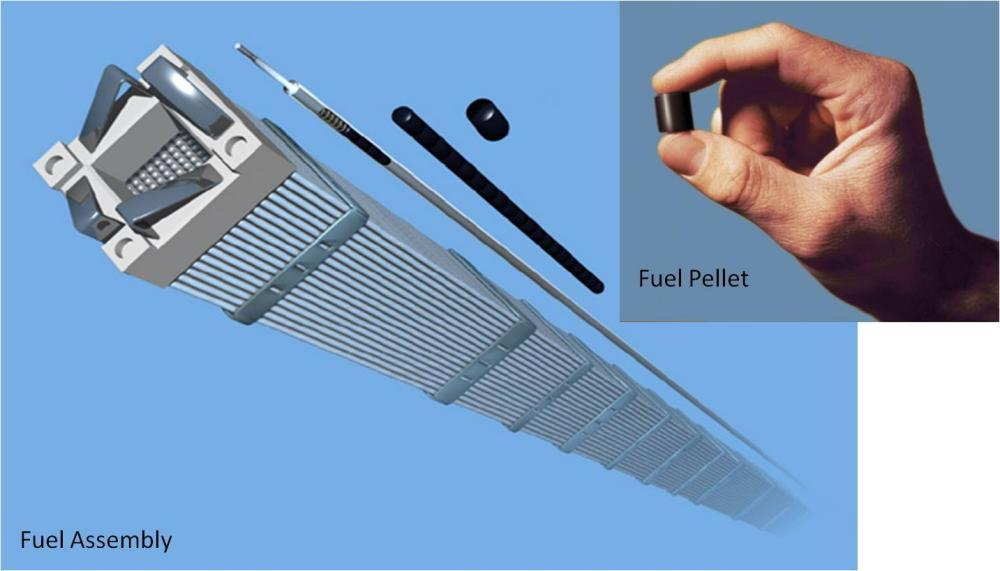
\includegraphics[width=0.95\textwidth]{pellet.jpg}
%        \caption{}
    \end{figure}
\end{frame}


\begin{frame}{}
    \begin{figure}
        \centering
        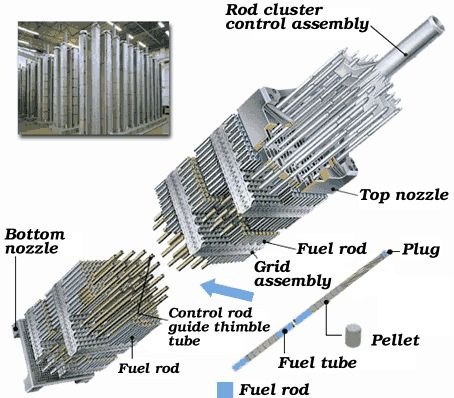
\includegraphics[width=0.55\textwidth]{pwr.jpg}
%        \caption{}
    \end{figure}
\end{frame}


\begin{frame}{}
    \begin{figure}
        \centering
        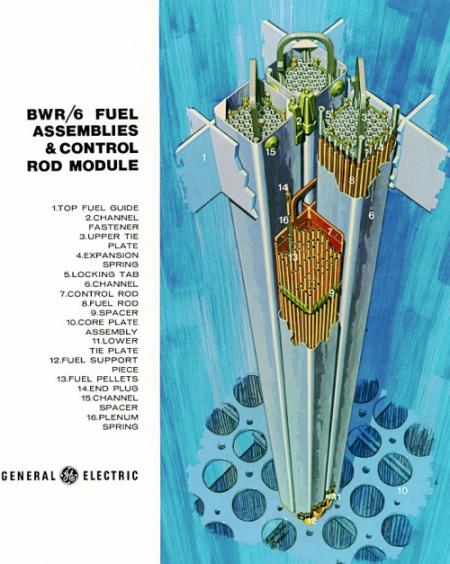
\includegraphics[width=0.35\textwidth]{bwr.jpg}
%        \caption{}
    \end{figure}
\end{frame}


\begin{frame}[plain]{}
    \centering\LARGE\textbf{Macro reactor operation}
\end{frame}


\begin{frame}[plain]{}
    \centering\LARGE\textbf{\acf{cp1}}
\end{frame}


\addtocounter{framenumber}{-2} 
\begin{frame}{The first man made reactor was constructed at \href{https://uidaho.pressbooks.pub/nuclearengineering/chapter/front-end-of-the-fuel-cycle-2/}{University of Chicago} in 1942}
    \begin{columns}[c]

        \begin{column}{0.55\textwidth}
            \begin{figure}
                \centering
                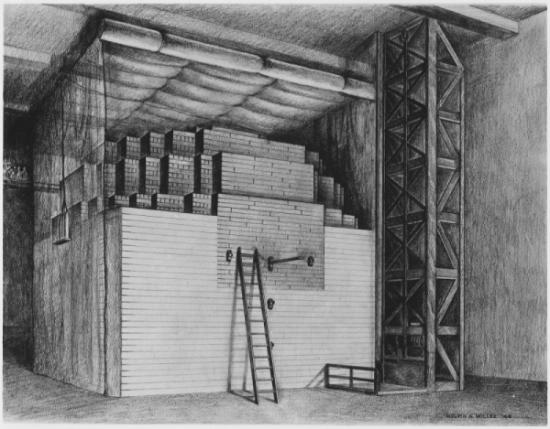
\includegraphics[width=0.95\textwidth]{cp1.jpg}
                %\caption{}
            \end{figure}
        \end{column}

        \begin{column}{0.45\textwidth}
            \begin{enumerate}[series=outerlist,topsep=0pt,itemsep=21pt,leftmargin=*,label=(\arabic*)]
                \item[]Made of uranium and graphite blocks
                \item[]Cadmium coated rods
                \item[]And I have a piece of the graphite
            \end{enumerate}
        \end{column}

    \end{columns}
\end{frame}


\begin{frame}[plain]{}
    \centering\LARGE\textbf{Let's look at pictures of the \href{https://uidaho.pressbooks.pub/nuclearengineering/chapter/front-end-of-the-fuel-cycle-2/}{Hanford B reactor}}\\
    \centering\large\textbf{Same design as CP1}
\end{frame}


\addtocounter{framenumber}{-1} 
\begin{frame}{}
    \begin{figure}
        \centering
        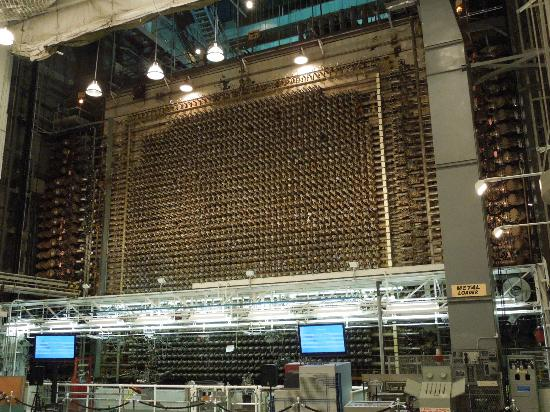
\includegraphics[width=0.75\textwidth]{hb1.jpg}
%        \caption{}
    \end{figure}
\end{frame}


\begin{frame}{}
    \begin{figure}
        \centering
        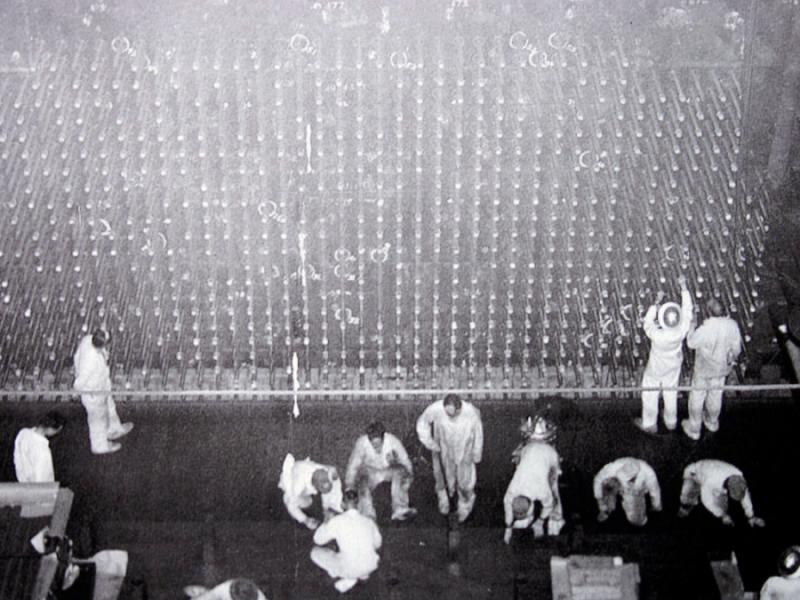
\includegraphics[width=0.75\textwidth]{hb2.jpg}
%        \caption{}
    \end{figure}
\end{frame}


\begin{frame}{}
    \begin{figure}
        \centering
        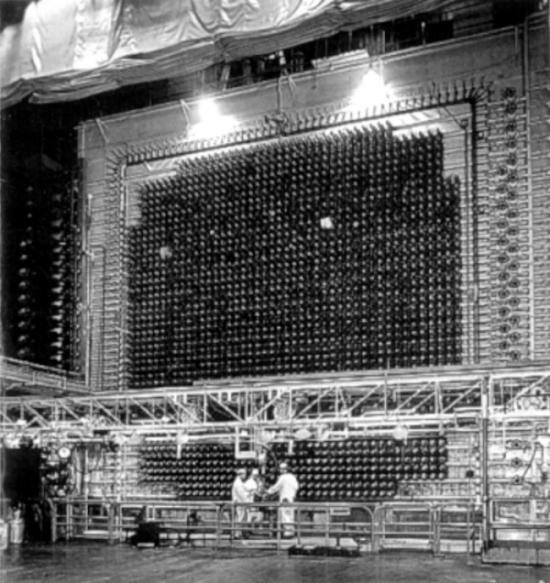
\includegraphics[width=0.55\textwidth]{hb3.jpg}
%        \caption{}
    \end{figure}
\end{frame}


\begin{frame}{}
    \begin{figure}
        \centering
        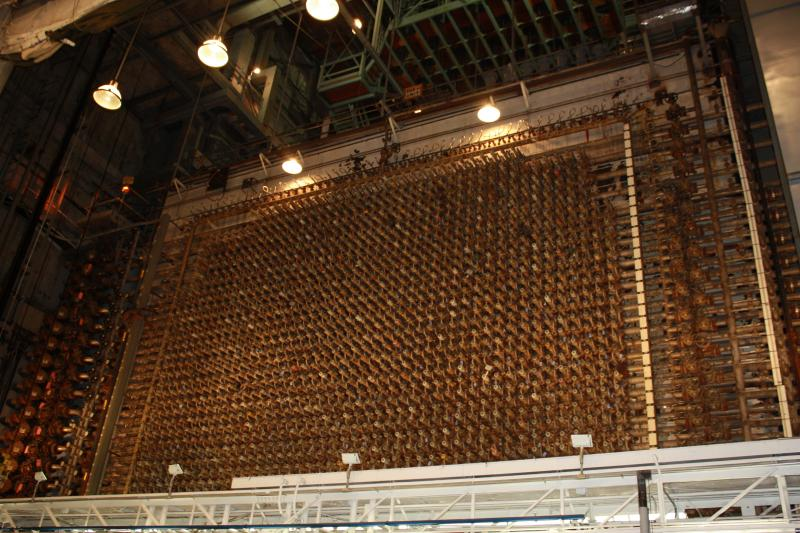
\includegraphics[width=0.55\textwidth]{hb4.jpg}
%        \caption{}
    \end{figure}
\end{frame}


\begin{frame}{}
    \begin{figure}
        \centering
        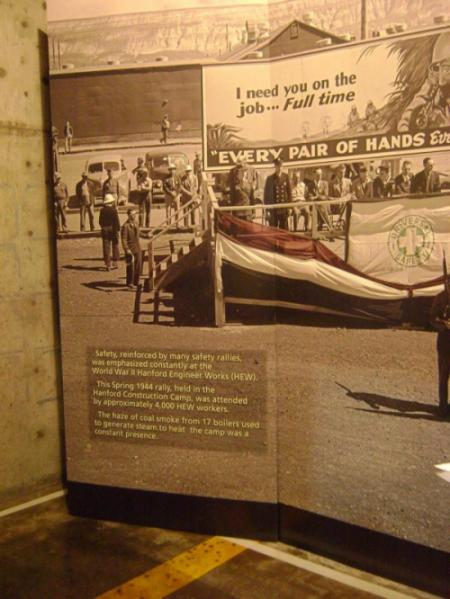
\includegraphics[width=0.45\textwidth]{hb5.jpg}
%        \caption{}
    \end{figure}
\end{frame}


\begin{frame}{}
    \begin{figure}
        \centering
        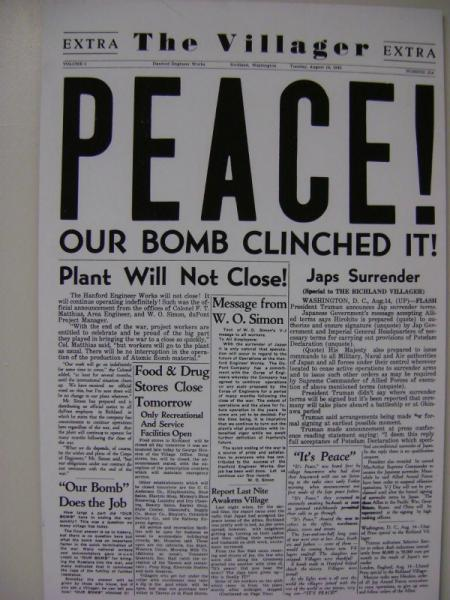
\includegraphics[width=0.45\textwidth]{hb6.jpg}
%        \caption{}
    \end{figure}
\end{frame}


\begin{frame}{}
    \begin{figure}
        \centering
        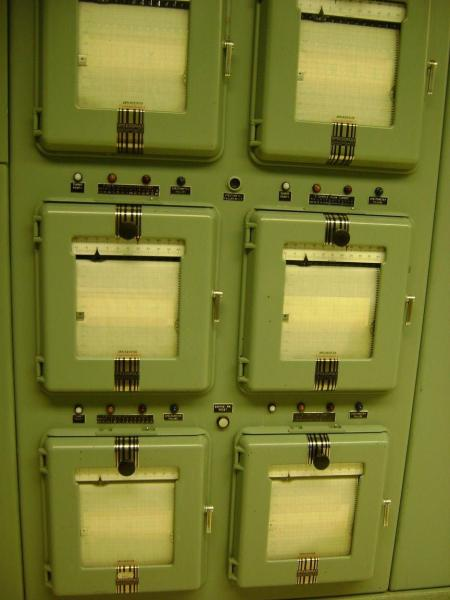
\includegraphics[width=0.45\textwidth]{hb7.jpg}
%        \caption{}
    \end{figure}
\end{frame}


\begin{frame}{}
    \begin{figure}
        \centering
        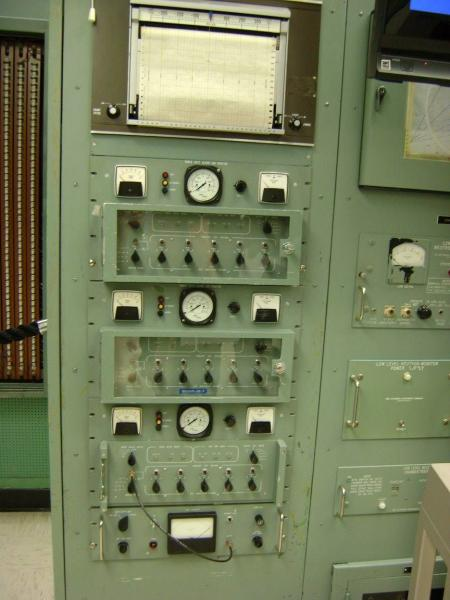
\includegraphics[width=0.45\textwidth]{hb8.jpg}
%        \caption{}
    \end{figure}
\end{frame}


\begin{frame}{}
    \begin{figure}
        \centering
        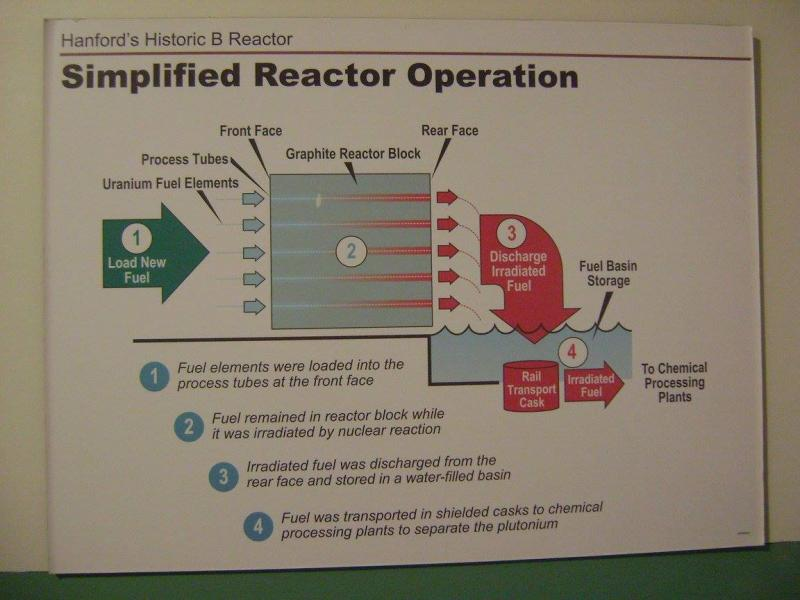
\includegraphics[width=0.55\textwidth]{hb9.jpg}
%        \caption{}
    \end{figure}
\end{frame}


\begin{frame}{}
    \begin{figure}
        \centering
        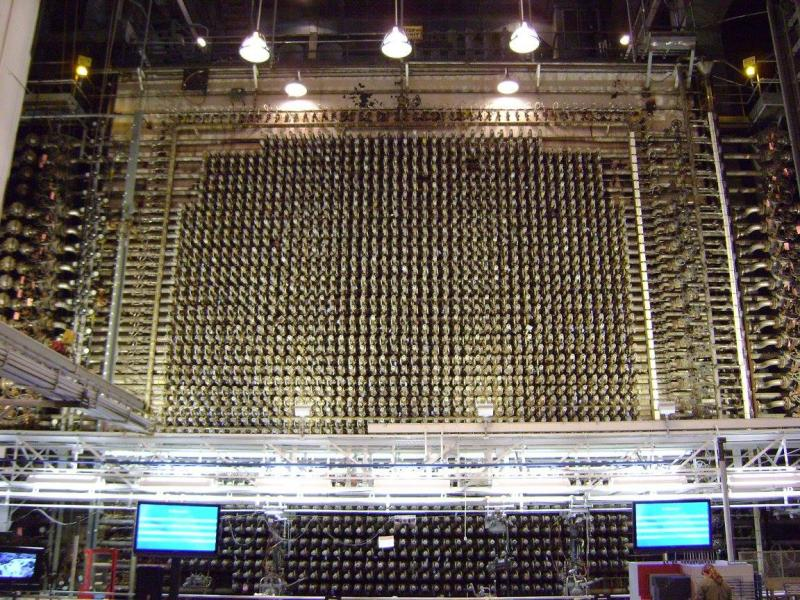
\includegraphics[width=0.55\textwidth]{hb10.jpg}
%        \caption{}
    \end{figure}
\end{frame}


\begin{frame}{}
    \begin{figure}
        \centering
        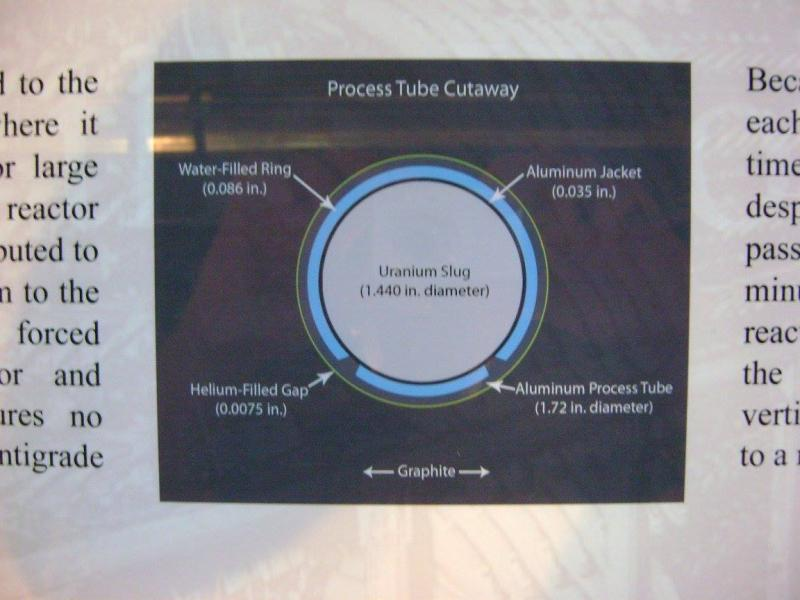
\includegraphics[width=0.55\textwidth]{hb11.jpg}
%        \caption{}
    \end{figure}
\end{frame}


\begin{frame}{}
    \begin{figure}
        \centering
        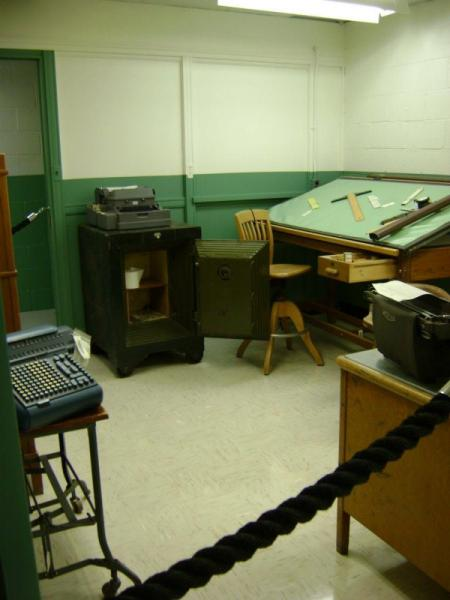
\includegraphics[width=0.45\textwidth]{hb12.jpg}
%        \caption{}
    \end{figure}
\end{frame}


\begin{frame}{}
    \begin{figure}
        \centering
        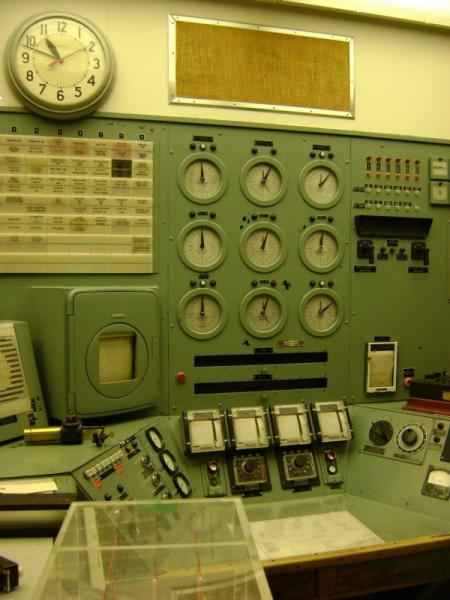
\includegraphics[width=0.45\textwidth]{hb13.jpg}
%        \caption{}
    \end{figure}
\end{frame}


\begin{frame}{}
    \begin{figure}
        \centering
        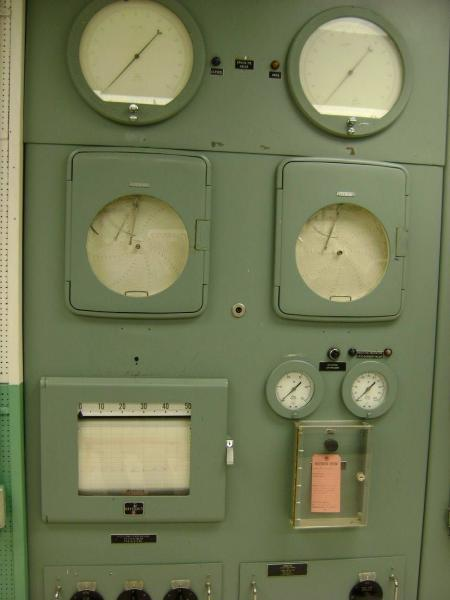
\includegraphics[width=0.45\textwidth]{hb14.jpg}
%        \caption{}
    \end{figure}
\end{frame}


\begin{frame}{}
    \begin{figure}
        \centering
        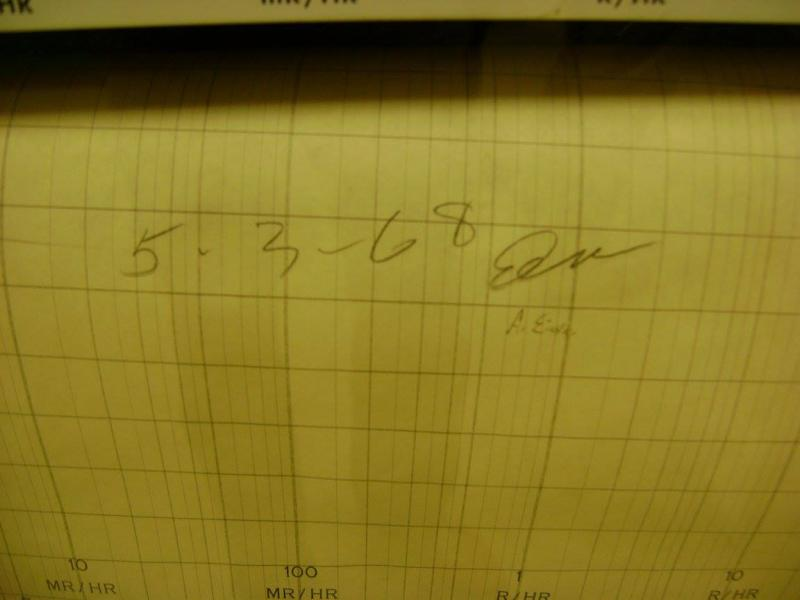
\includegraphics[width=0.75\textwidth]{hb15.jpg}
%        \caption{}
    \end{figure}
\end{frame}


\begin{frame}[plain]{}
    \centering\LARGE\textbf{Natural reactor}
\end{frame}


\addtocounter{framenumber}{-1} 
\begin{frame}{A \href{https://uidaho.pressbooks.pub/nuclearengineering/chapter/nuclear-fuel-cycle-system/}{natural reactor} actually happened about \href{https://uidaho.pressbooks.pub/nuclearengineering/chapter/neutronics/}{2 billion years ago}}
    \begin{enumerate}[series=outerlist,topsep=0pt,itemsep=21pt,leftmargin=*,label=(\arabic*)]
        \item[]16 sites operated for about $10^5$ years at 100 kW thermal
        \item[]French company found samples of 0.60\% of $^{235}U$
        \item[]How much is there normally?
        \item[]Uranium rich mineral deposits were infiltrated by groundwater which served as moderator
    \end{enumerate}
\end{frame}


\begin{frame}{}
    \begin{figure}
        \centering
        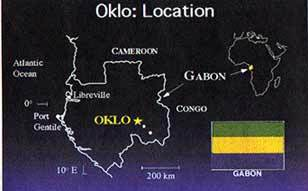
\includegraphics[width=0.75\textwidth]{oklo.location.jpg}
%        \caption{}
    \end{figure}
\end{frame}


\begin{frame}{}
    \begin{figure}
        \centering
        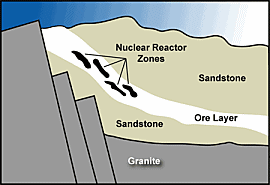
\includegraphics[width=0.75\textwidth]{oklo.jpg}
%        \caption{}
    \end{figure}
\end{frame}


\begin{frame}[plain]{}
    \centering\LARGE\textbf{\acs{eb1}}
\end{frame}


\addtocounter{framenumber}{-1} 
\begin{frame}{\href{https://uidaho.pressbooks.pub/nuclearengineering/chapter/nuclear-fuel-cycle-system/}{\acs{eb1}} was the first reactor to \href{https://uidaho.pressbooks.pub/nuclearengineering/chapter/fuel-cycle-analysis/}{generate electricity}}
    \begin{enumerate}[series=outerlist,topsep=0pt,itemsep=21pt,leftmargin=*,label=(\arabic*)]
        \item[]In 1951 - now a \href{https://inl.gov/experimental-breeder-reactor-i/}{museum}, open to the public for free
        \item[]About 200 kW of electricity
        \item[]Also was a breeder and first to confirm Fermi’s theory
        \item[]`Fast' reactor, metal fuel and molten salt designs
        \item[]Then the commercial reactors switched to ceramic and water
        \item[]Why?
        \item[]Now the so called Generation IV reactor designs use metals and salts 
    \end{enumerate}
\end{frame}


\begin{frame}{}
    \begin{figure}
        \centering
        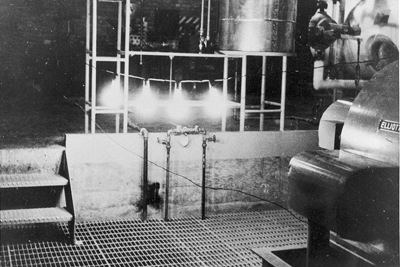
\includegraphics[width=0.75\textwidth]{ebr1.light.jpg}
%        \caption{}
    \end{figure}
\end{frame}


\begin{frame}[plain]{}
    \centering\LARGE\textbf{More pictures}
\end{frame}


\addtocounter{framenumber}{-1} 
\begin{frame}{}
    \begin{figure}
        \centering
        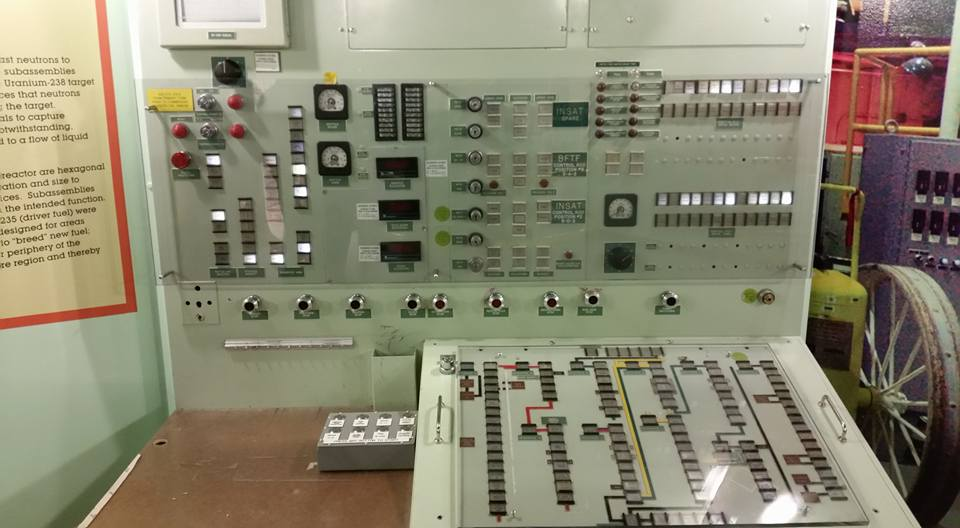
\includegraphics[width=0.75\textwidth]{ebr1.jpg}
%        \caption{}
    \end{figure}
\end{frame}


\begin{frame}{}
    \begin{figure}
        \centering
        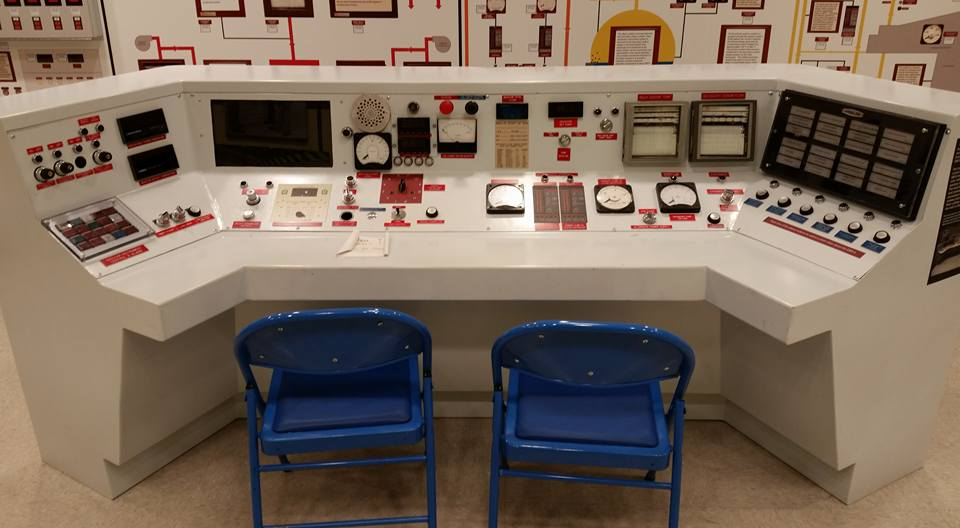
\includegraphics[width=0.75\textwidth]{ebr2.jpg}
%        \caption{}
    \end{figure}
\end{frame}


\begin{frame}{}
    \begin{figure}
        \centering
        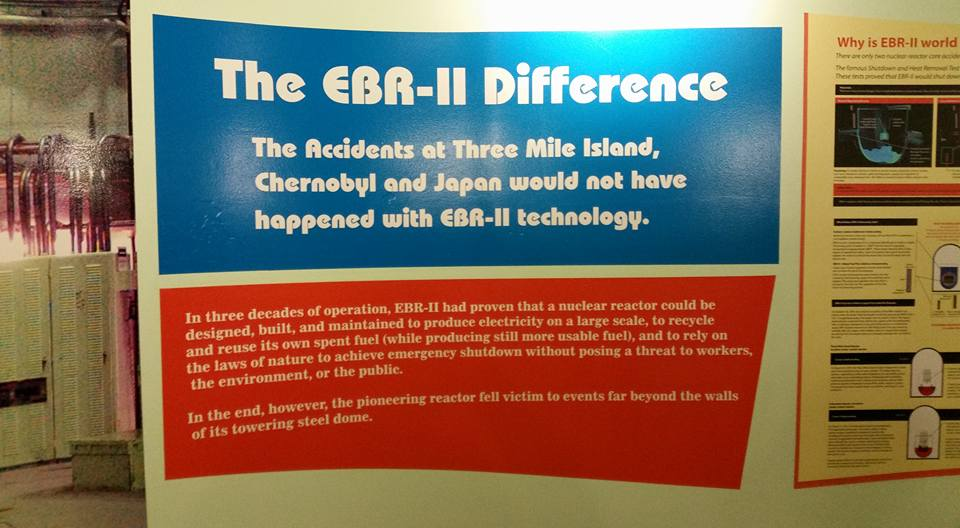
\includegraphics[width=0.75\textwidth]{ebr3.jpg}
%        \caption{}
    \end{figure}
\end{frame}


\begin{frame}{}
    \begin{figure}
        \centering
        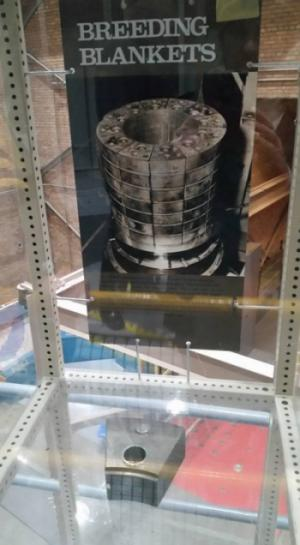
\includegraphics[width=0.25\textwidth]{ebr4.jpg}
%        \caption{}
    \end{figure}
\end{frame}


\begin{frame}{}
    \begin{figure}
        \centering
        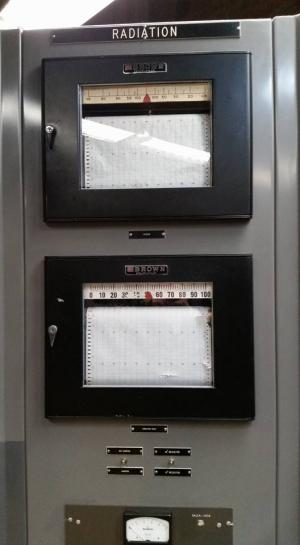
\includegraphics[width=0.25\textwidth]{ebr5.jpg}
%        \caption{}
    \end{figure}
\end{frame}


\begin{frame}{}
    \begin{figure}
        \centering
        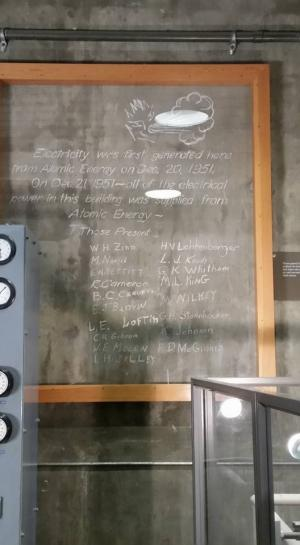
\includegraphics[width=0.25\textwidth]{ebr6.jpg}
%        \caption{}
    \end{figure}
\end{frame}


\begin{frame}{}
    \begin{figure}
        \centering
        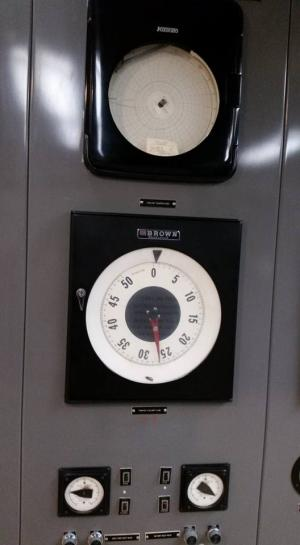
\includegraphics[width=0.25\textwidth]{ebr7.jpg}
%        \caption{}
    \end{figure}
\end{frame}


\begin{frame}{}
    \begin{figure}
        \centering
        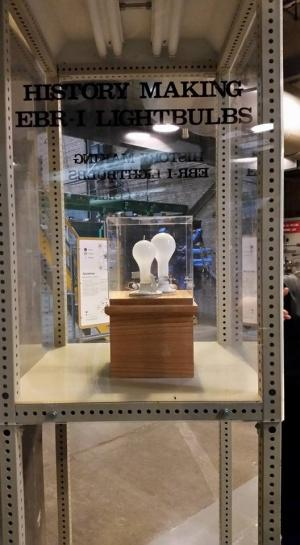
\includegraphics[width=0.25\textwidth]{ebr8.jpg}
%        \caption{}
    \end{figure}
\end{frame}


\begin{frame}{}
    \begin{figure}
        \centering
        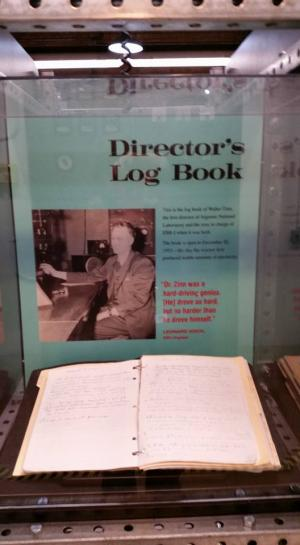
\includegraphics[width=0.25\textwidth]{ebr9.jpg}
%        \caption{}
    \end{figure}
\end{frame}


\begin{frame}{}
    \begin{figure}
        \centering
        \includegraphics[width=0.75\textwidth]{ebr10.jpg}
%        \caption{}
    \end{figure}
\end{frame}


\begin{frame}{}
    \begin{figure}
        \centering
        \includegraphics[width=0.25\textwidth]{ebr11.jpg}
%        \caption{}
    \end{figure}
\end{frame}


\begin{frame}{}
    \begin{figure}
        \centering
        \includegraphics[width=0.75\textwidth]{ebr12.jpg}
%        \caption{}
    \end{figure}
\end{frame}


\begin{frame}{}
    \begin{figure}
        \centering
        \includegraphics[width=0.75\textwidth]{ebr13.jpg}
%        \caption{}
    \end{figure}
\end{frame}


\begin{frame}{}
    \begin{figure}
        \centering
        \includegraphics[width=0.75\textwidth]{ebr14.jpg}
%        \caption{}
    \end{figure}
\end{frame}


\begin{frame}[plain]{}
    \centering\LARGE\textbf{\acs{eb2}}
\end{frame}


\addtocounter{framenumber}{-1} 
\begin{frame}{\acs{eb2} is an \acf{sfr} design for 62.5 MW that operated from 1964 to 1994}
    \begin{enumerate}[series=outerlist,topsep=0pt,itemsep=21pt,leftmargin=*,label=(\arabic*)]
        \item[]19 MW electricity operated for 30 years with no accidents
        \item[]Engineering scale facility
        \item[]Breeder reactor with onsite reprocessing (pyroprocessing)
        \item[]Famous test of \href{https://youtu.be/Sp1Xja6HlIU}{passive safety systems}
    \end{enumerate}
\end{frame}


\begin{frame}{}
    \begin{figure}
        \centering
        \includegraphics[width=0.35\textwidth]{ebrii.jpg}
%        \caption{}
    \end{figure}
\end{frame}


\begin{frame}[plain]{}
    \centering\LARGE\textbf{\acs{trt}}
\end{frame}


\addtocounter{framenumber}{-1} 
\begin{frame}{\href{https://uidaho.pressbooks.pub/nuclearengineering/chapter/front-end-of-the-fuel-cycle/}{\acs{trt}} is an air cooled, graphite moderated thermal reactor}
    \begin{enumerate}[series=outerlist,topsep=0pt,itemsep=21pt,leftmargin=*,label=(\arabic*)]
        \item[]Operation from 1959 to 1994
        \item[]Transient reactor tests to simulate all sorts of reactor accidents
        \item[]George Imel
        \item[]Restarted and working on experiments!
        \item[]Because of Fukushima, \acs{trt} accident tolerant fuels
        \item[]Everyone is excited
        \item[]100 kW; transients up to 19 GW
    \end{enumerate}
\end{frame}


\begin{frame}{}
    \begin{figure}
        \centering
        \includegraphics[width=0.75\textwidth]{treat.jpg}
%        \caption{}
    \end{figure}
\end{frame}


\begin{frame}[plain]{}
    \centering\LARGE\textbf{Military use}
\end{frame}


\addtocounter{framenumber}{-1} 
\begin{frame}{Nuclear reactors are used on submarines and aircraft carriers}
    \begin{enumerate}[series=outerlist,topsep=0pt,itemsep=21pt,leftmargin=*,label=(\arabic*)]
        \item[]\href{https://www.independent.co.uk/life-style/history/a-day-that-shook-the-world-first-nuclear-submarine-launched-2189571.html}{Nautilus launched in 1954}
        \item[]25 year life span
        \item[]Nimitz-class aircraft carriers have 2 reactors, about 100 MW, 23 year life span
        \item[]How about now?
    \end{enumerate}
\end{frame}


\begin{frame}{}
    \begin{figure}
        \centering
        \includegraphics[width=0.75\textwidth]{nautilus.jpg}
%        \caption{}
    \end{figure}
\end{frame}


\begin{frame}{}
    \begin{figure}
        \centering
        \includegraphics[width=0.75\textwidth]{carrier.jpg}
        \caption*{Watch out for the \href{https://youtu.be/siwpn14IE7E}{danger zone}}
    \end{figure}
\end{frame}


\begin{frame}[plain]{}
    \centering\LARGE\textbf{Reactor concepts}
\end{frame}


\begin{frame}[plain]{}
    \centering\LARGE\textbf{Generations}
\end{frame}


\addtocounter{framenumber}{-2} 
\begin{frame}{Reactors were first built in the 1950s}
    \begin{columns}[t]

        \begin{column}{0.55\textwidth}
            \begin{figure}
                \centering
                \includegraphics[width=0.95\textwidth]{generation.jpg}
                %\caption{}
            \end{figure}
        \end{column}

        \begin{column}{0.45\textwidth}
            \begin{enumerate}[series=outerlist,topsep=0pt,itemsep=21pt,leftmargin=*,label=(\arabic*)]
                \item[]Gen IV is essentially based on Gen I
                \item[]Different material for fuels and coolant
                \item[]Moderators not needed for some
                \item[]Passive safety systems
                \item[]Proliferation issues -- so they say
            \end{enumerate}
        \end{column}

    \end{columns}
\end{frame}


\begin{frame}[plain]{}
    \centering\LARGE\textbf{\acs{pwr}}
\end{frame}


\addtocounter{framenumber}{-1} 
\begin{frame}{The \acs{pwr} heats water but does not boil}
    \begin{figure}
        \centering
        \includegraphics[width=0.75\textwidth]{pwr.system.jpg}
%        \caption{}
    \end{figure}
\end{frame}


\begin{frame}[plain]{}
    \centering\LARGE\textbf{\acs{bwr}}
\end{frame}


\addtocounter{framenumber}{-1} 
\begin{frame}{The \acs{bwr} does boil water in the reactor vessel}
    \begin{figure}
        \centering
        \includegraphics[width=0.75\textwidth]{bwr.system.jpg}
%        \caption{}
    \end{figure}
\end{frame}


\begin{frame}[plain]{}
    \centering\LARGE\textbf{\acs{cdu}}
\end{frame}


\addtocounter{framenumber}{-1} 
\begin{frame}{The \acs{cdu} design uses heavy water (moderator) and natural uranium (also thermal)}
    \begin{figure}
        \centering
        \includegraphics[width=0.75\textwidth]{CANDU.jpg}
%        \caption{}
    \end{figure}
\end{frame}


\begin{frame}{More on \acs{cdu}}
    \begin{enumerate}[series=outerlist,topsep=0pt,itemsep=18pt,leftmargin=*,label=(\arabic*)]
        \item[]Used in Canada and marketed to other nations
        \item[]South Korea, China, India have some
        \item[]\acs{pwr} design (two loops)
        \item[]The heavy water is less absorbing so natural U can be used
        \item[]But also more collisions would be needed than in \acsp{lwr}
        \item[]The core would be bigger
        \item[]But can use used fuel from \acsp{lwr} and a Th cycle
        \item[]So is there an advantage?  Technical?  Institutional?
    \end{enumerate}
\end{frame}


\begin{frame}{The \acs{cdu} design uses heavy water (moderator) and natural uranium (also thermal)}
    \begin{figure}
        \centering
        \includegraphics[width=0.55\textwidth]{simpsons.jpg}
%        \caption{}
    \end{figure}
\end{frame}


\begin{frame}[plain]{}
    \centering\LARGE\textbf{Aqueous reprocessing}
\end{frame}


\addtocounter{framenumber}{-1} 
\begin{frame}{Aqueous recycling is the \href{https://uidaho.pressbooks.pub/nuclearengineering/chapter/countercurrent-solvent-extraction/}{commercially available} process for \acsp{lwr}}
    \begin{enumerate}[series=outerlist,topsep=0pt,itemsep=18pt,leftmargin=*,label=(\arabic*)]
        \item[]Terry Todd leading expert
        \item[]Major nations are France, Japan, Russia, India
        \item[]`Recycle' is better for the brand
        \item[]About 1\% 235U and 1\% Pu in used fuel
        \item[]The most common is \acs{pur}
        \item[]This uses an organic phosphate and nitric acid
        \item[]Solvent extraction process where U and Pu are separated
        \item[]Then created into \acs{mox} fuel
        \item[]So for \acs{pur} what is a big risk?
    \end{enumerate}
\end{frame}


\begin{frame}{}
    \begin{figure}
        \centering
        \includegraphics[width=0.50\textwidth]{purex.jpg}
%        \caption{}
    \end{figure}
\end{frame}


\begin{frame}{U and Pu are chemically separated through organic solvent equilibrium extraction}
    \begin{enumerate}[topsep=0pt,itemsep=11pt,leftmargin=*,label=(\arabic*)]
        \item[]U and Pu exist in a number of valence states
        \item[]Because of different redox potentials, reduction or oxidation can be done to one without disturbing the other
        \item[]Each exhibits different solubilities in organic solvent \acs{tbp}
    \end{enumerate}

    \vspace{0.25in}
    
    \begin{enumerate}[topsep=0pt,itemsep=7pt,leftmargin=*,label=(\arabic*)]
        \item Chop up everything, remove \acs{fp} gases, dissolve in aqueous solution
        \item Separate U/Pu from fission products by dissolving in solvent
        \item Reduce Pu to 3+ because it is highly insoluble in solvent (U 6+)
        \item Back extract Pu into aqueous solution  
        \item Strip U from solvent into aqueous solution
    \end{enumerate}
\end{frame}


\begin{frame}{U and Pu are chemically separated through organic solvent equilibrium extraction}
    \begin{enumerate}[topsep=0pt,itemsep=21pt,leftmargin=*,label=(\arabic*)]
        \item[]Aqueous solution is nitric acid
        \item[]Does generate a lot of liquid waste
        \item[]Mass transfer to solvent phase -- extraction  
        \item[]Mass transfer to aqueous phase --`` stripping
    \end{enumerate}
\end{frame}


\begin{frame}{Mass transfer operates in a continuous, multistage, countercurrent mode}
    \begin{enumerate}[topsep=0pt,itemsep=21pt,leftmargin=*,label=(\arabic*)]
        \item[]High separation factor
        \item[]High processing rates
        \item[]Streams flow countercurrently, so concentration is relatively constant
        \item[]Solvent must be recycled because it's not cheap
        \item[]First applied to extract Pu for weapons production in 1952 at Hanford site
    \end{enumerate}
\end{frame}


\begin{frame}{Metals in 4+ and 6+ are extracted}
    \begin{equation}
        \Large
        (UO_2)^{2+}(aq) + 2(NO_3)^-(aq) + 2TPB(o) \leftrightarrow UO_2(NO_3)_2 \cdot 2TBP(o)
    \end{equation}
    
    \begin{equation}
        \Large
        An^{4+}(aq) + 4NO_3^-(aq) + 2TBP(o) \leftrightarrow An_2(NO_3)_4 \cdot 2TBP(o)
    \end{equation}

    \vspace*{\fill}

    \begin{enumerate}[topsep=0pt,itemsep=18pt,leftmargin=*,label=(\arabic*)]
        \item[]Pu (as 4+) co-extracted with U
        \item[]Anything 3+ or lower is not
        \item[]Waste is vitrified into a borosilicate glass waste form for disposal
        \item[]Well characterized material with 50+ years of scientific study
        \item[]Very stable
    \end{enumerate}
\end{frame}


\begin{frame}{}
    \begin{figure}
        \centering
        \includegraphics[width=0.95\textwidth]{purex.flow.jpg}
%        \caption{}
    \end{figure}
\end{frame}


\begin{frame}{Typical mass conservation is used to model \href{https://uidaho.pressbooks.pub/nuclearengineering/chapter/countercurrent-solvent-extraction/}{solvent extraction}}
    
    \begin{enumerate}[topsep=0pt,itemsep=18pt,leftmargin=*,label=(\arabic*)]
        \item[]This is from Benedict
        \item[]Distribution coefficient = organic/aqueous phase concentration at equilibrium
    \end{enumerate}

    \vspace*{\fill}

    \begin{equation}
        \LARGE
        D \equiv \frac{y}{x}
    \end{equation}

    \vspace*{\fill}

    \begin{enumerate}[topsep=0pt,itemsep=18pt,leftmargin=*,label=(\arabic*)]
        \item[]When an aqueous solution of an extractable component is brought into equilibrium with an immiscible solvent for the component and the two phases are then separated, the component will be found distributed between the two phases
    \end{enumerate}
\end{frame}


\begin{frame}{We then derive the material balance on the extractable component}
    \begin{equation}
        \LARGE
        Fz = Fx + Ey
    \end{equation}
    
    \vspace*{\fill}

    \begin{enumerate}[topsep=0pt,itemsep=18pt,leftmargin=*,label=(\arabic*)]
        \item[]With $D$ for the system defined before
    \end{enumerate}
\end{frame}


\begin{frame}{}
    \begin{figure}
        \centering
        \includegraphics[width=0.90\textwidth]{single.stage.jpg}
%        \caption{}
    \end{figure}
\end{frame}


\begin{frame}{Derive the concentration that is extracted}
    \begin{equation}
        \LARGE
        D \equiv \frac{y}{x}
    \end{equation}
    
    \begin{equation}
        \LARGE
        Fz = Fx + Ey
    \end{equation}
    
    \begin{equation}
        \LARGE
        \therefore y = \frac{Dz}{1+\frac{ED}{F}}
    \end{equation}
    
    \vspace*{\fill}

    \begin{enumerate}[topsep=0pt,itemsep=18pt,leftmargin=*,label=(\arabic*)]
        \item[]And the fraction extracted is -- 
    \end{enumerate}

    \vspace*{\fill}

    \begin{equation}
        \LARGE
        \rho = \frac{Ey}{Fz} = \frac{1}{1+\frac{F}{ED}}
    \end{equation}

    \vspace*{\fill}

    \begin{enumerate}[topsep=0pt,itemsep=18pt,leftmargin=*,label=(\arabic*)]
        \item[]For design then, you only need 3 parameters
    \end{enumerate}
\end{frame}


\begin{frame}{Derive the solvent feed needed for a given extraction fraction}
    \begin{equation}
        \LARGE
        \frac{E}{F} = \frac{\rho}{D(1 - \rho)}
    \end{equation}
    
    \vspace*{\fill}

    \begin{enumerate}[topsep=0pt,itemsep=21pt,leftmargin=*,label=(\arabic*)]
        \item[]What is the functional dependence of $E(\rho)$?
        \item[]Amount of used fuel isn't actually a variable 
    \end{enumerate}
\end{frame}


\begin{frame}{Reduce the amount of solvent by using multiple contact stages}
    \begin{enumerate}[topsep=0pt,itemsep=21pt,leftmargin=*,label=(\arabic*)]
        \item[]With many stages, high extraction fraction can be obtained
        \item[]Solvent is expensive, so recycling stages are also added to strip out extract
        \item[]Multiple components can be extracted from organic phase if $D$ is different enough
        \item[]So this would be needed to completely separate U, Pu
        \item[]Physical conditions affecting $D$ --
            \begin{enumerate}[topsep=0pt,itemsep=3pt,leftmargin=*,label=(\arabic*)]
                \item[]Element extracted
                \item[]Redox potential of aqueous phase
                \item[]Solvent
                \item[]Concentrations
                \item[]$[H^+]_{aq}$
            \end{enumerate}
    \end{enumerate}
\end{frame}


\begin{frame}{}
    \begin{figure}
        \centering
        \includegraphics[width=0.50\textwidth]{purex.jpg}
%        \caption{}
    \end{figure}
\end{frame}


\begin{frame}{}
    \begin{figure}
        \centering
        \includegraphics[width=0.75\textwidth]{multistage.jpg}
%        \caption{}
    \end{figure}
\end{frame}


\begin{frame}{}
    \begin{figure}
        \centering
        \includegraphics[width=0.75\textwidth]{engineering.flow.jpg}
%        \caption{}
    \end{figure}
\end{frame}


\begin{frame}{Now apply same mass conservation to multistage extraction}
    \begin{enumerate}[topsep=0pt,itemsep=21pt,leftmargin=*,label=(\arabic*)]
        \item[]Assume equilibrium between phases
        \item[]Material balance on extractable component below stage $n$ --
    \end{enumerate}

    \vspace*{\fill}

    \begin{equation}
        \LARGE
        Ey_0 + Fx_n = Ey_{n-1} + Fx_1
    \end{equation}

    \begin{equation}
        \LARGE
        y_{n-1} - y_0 = \frac{F}{E}(x_n-x_1)
    \end{equation}
    
    \vspace*{\fill}

    \begin{enumerate}[topsep=0pt,itemsep=18pt,leftmargin=*,label=(\arabic*)]
        \item[]$\therefore$ for any stage -- 
    \end{enumerate}

    \vspace*{\fill}

    \begin{equation}
        \LARGE
        y_n \equiv D_nx_n
    \end{equation}
\end{frame}


\begin{frame}{\href{http://ljs.academicdirect.org/A20/079_094.pdf}{McCabe-Thiele diagram} can be used for constructing graphical solution for for stage concentrations}
    \begin{enumerate}[topsep=0pt,itemsep=21pt,leftmargin=*,label=(\arabic*)]
        \item[]Basically gives the number of stages for an extraction concentration $x_F$
        \item[]By graphing $y_{n-1} - y_0 = \frac{F}{E}(x_n-x_1)$ on $y$ versus $x$
        \item[]Construct operating line to satisfy the above and pass through $x_1,y_0$ with slope $\frac{F}{E}$ relative to equilibrium line $y_n = D_nx_n$
        \item[]Cannot really change equilibrium line because it is based on $D$
        \item[]Reduce the concentration of the extractable component from $x_F$ to $x_1$ with $\frac{F}{E}$
        \item[]Start at $x_1,y_0$ and move up
    \end{enumerate}
\end{frame}


\begin{frame}{}
    \begin{figure}
        \centering
        \href{http://www.tsijournals.com/articles-images/chemical-technology-McCabe-Thiele-uranium-11-5-102-g015.png}{\includegraphics[width=0.70\textwidth]{mccabe.jpg}}
%        \caption{}
    \end{figure}
\end{frame}


\begin{frame}{Derive the extraction factor for multiple stages}
    \begin{equation}
        \LARGE
        \rho \equiv \frac{Ey_N}{Fx_F}
    \end{equation}
    
    \vspace*{\fill}

    \begin{enumerate}[topsep=0pt,itemsep=18pt,leftmargin=*,label=(\arabic*)]
        \item[]Or -- 
    \end{enumerate}

    \vspace*{\fill}

    \begin{equation}
        \LARGE
        1 - \rho = \frac{x_1}{x_F}
    \end{equation}

    \vspace*{\fill}

    \begin{enumerate}[topsep=0pt,itemsep=18pt,leftmargin=*,label=(\arabic*)]
        \item[]What does this tell us?
        \item[]And feed ratio can be defined in terms of $f(\rho)$ as --
    \end{enumerate}

    \vspace*{\fill}

    \begin{equation}
        \LARGE
        \frac{E}{F} = \frac{\rho x_F}{y_N-y_0}
    \end{equation}
\end{frame}


\begin{frame}[plain]{}
    \centering\LARGE\textbf{How many stages for complete extraction?}\\
    \centering\LARGE\textbf{What does that look like on McCabe-Thiele?}
\end{frame}


\addtocounter{framenumber}{-1} 
\begin{frame}{Apply these concepts to model multistage extraction based on \href{http://wwwcourses.sens.buffalo.edu/ce407/notes/ce407_notes_Lecture03.pdf}{Kremser equation}}
    \begin{equation}
        \Large
        y_{n-1} - y_0 = \frac{F}{E}(x_n-x_1)
    \end{equation}
    
    \begin{equation}
        \Large
        y_n \equiv D_nx_n
    \end{equation}
    
    \begin{equation}
        \Large
        \beta \equiv \frac{DE}{F}
    \end{equation}
    
    \vspace*{\fill}

    \begin{enumerate}[topsep=0pt,itemsep=1pt,leftmargin=*,label=(\arabic*)]
        \item[]Then -- 
    \end{enumerate}

    \vspace*{\fill}

    \begin{equation}
        \Large
        y_n = \beta (y_{n-1} - y_0) + Dx_1
    \end{equation}

    \begin{equation}
        \Large
        y_N = \frac{\beta^N - 1}{\beta - 1}(Dx_1-y_0) +y_0
    \end{equation}
\end{frame}


\begin{frame}{This can also be applied if there are two extractable components in the feed}
    \begin{equation}
        \LARGE
        D_A \; D_B \; \beta_A \; \beta_B
    \end{equation}
    
    \vspace*{\fill}

    \begin{enumerate}[topsep=0pt,itemsep=18pt,leftmargin=*,label=(\arabic*)]
        \item[]Define decontamination factor. What does this mean?
    \end{enumerate}

    \vspace*{\fill}

    \begin{equation}
        \LARGE
        f_{AB} \equiv \frac{\rho_A}{\rho_B}
    \end{equation}

    \begin{equation}
        \LARGE
        f_{AB} = \frac{\beta_A}{\beta_B}(\frac{\beta^N_A - 1}{\beta^N_B - 1})(\frac{\beta^{N+1}_B - 1}{\beta^{N+1}_A - 1}), \; y_0 = 0
    \end{equation}
\end{frame}


\begin{frame}[plain]{}
    \centering\LARGE\textbf{Conversion \& Enrichment}
\end{frame}


\addtocounter{framenumber}{-1} 
\begin{frame}{Uranium enrichment derived from World War II}
    \begin{enumerate}[topsep=0pt,itemsep=21pt,leftmargin=*,label=(\arabic*)]
        \item[]Needed to make bombs
        \item[]Then used the uranium for submarines 
        \item[]When moving to commercial power, infrastructure already in place
        \item[]Gaseous diffusion first invented at Oak Ridge
        \item[]Uranium hexafluoride used for enrichment
    \end{enumerate}
\end{frame}


\begin{frame}{Yellowcake needs to be purified first}
    \begin{enumerate}[topsep=0pt,itemsep=21pt,leftmargin=*,label=(\arabic*)]
        \item[]Impurities are rare earths, chlorine cadmium
        \item[]Uranium readily forms chemical compounds (lots of oxidation states)
        \item[]Can be extracted by organic solvents
        \item[]Uranium forms complexes that can be precipitated out
    \end{enumerate}
\end{frame}


\begin{frame}{There are different forms that are mined}
    \begin{equation}
        \LARGE
        \begin{aligned}
            & xUO_2 \cdot yUO_3
            \\
            & 0 < y/x < 2
        \end{aligned}
    \end{equation}
    
    \begin{equation}
        \LARGE
        K_2O \cdot 2UO_3 \cdot V_2O_5 \cdot xH_2O
    \end{equation}

    \begin{equation}
        \LARGE
        CaO \cdot 2UO_3 \cdot P_2O_5 \cdot xH_2O
    \end{equation}
    
    \vspace*{\fill}

    \begin{enumerate}[topsep=0pt,itemsep=18pt,leftmargin=*,label=(\arabic*)]
        \item[]Goal is to get it as $UO_3^{2+}$ and then acid or alkaline leaching
    \end{enumerate}

    \vspace*{\fill}

    \begin{equation}
        \LARGE
        UO_3 + 2H^+ \rightarrow UO_2^{2+} + H_2O
    \end{equation}

    \begin{equation}
        \LARGE
        UO_2 + 2Fe^{3+} \rightarrow UO_2^{2+} + 2Fe^{2+}
    \end{equation}
\end{frame}


\begin{frame}{Acid leaching is like \acs{pur} using organic solvent}
    \begin{equation}
        \LARGE
        UO_2^{2+} + 2NO_3 + 2TBP \rightarrow UO_2(NO_3)_2 \cdot 2TBP
    \end{equation}
    
    \begin{equation}
        \LARGE
        UO_2(NO_3)_2 + 2H_2O_2 + H_2O \rightarrow UO_4 \cdot 2H_2O + 2HNO_3
    \end{equation}

    \vspace*{\fill}

    \begin{enumerate}[topsep=0pt,itemsep=18pt,leftmargin=*,label=(\arabic*)]
        \item[]Precipitates uranium peroxide
    \end{enumerate}

    \vspace*{\fill}

    \begin{equation}
        \LARGE
        2Na_2S_2O_3 + UO_4 + H_2O \rightarrow Na_2S_4O_6 + UO_3 + 2NaOH
    \end{equation}
    
    \vspace*{\fill}

    \begin{enumerate}[topsep=0pt,itemsep=18pt,leftmargin=*,label=(\arabic*)]
        \item[]Or use ammonium hydroxide
    \end{enumerate}

    \vspace*{\fill}

    \begin{equation}
        \LARGE
        UO_2^{2+} + 6NH_4(OH) \rightarrow (NH_4)_2U_2O_7 + 4NH_4^+ + 3H_2O
    \end{equation}

    \vspace*{\fill}

    \begin{enumerate}[topsep=0pt,itemsep=11pt,leftmargin=*,label=(\arabic*)]
        \item[]Then dry and calcine to get $UO_3$
        \item[]If alkaline leaching is used, recover $U_3O_8$
    \end{enumerate}
\end{frame}


\begin{frame}{Uranium hexafluoride has favorable properties}
    \begin{columns}

        \begin{column}{0.45\textwidth}
            \begin{figure}
                \centering
                \includegraphics[width=0.95\textwidth]{uf6.phase.diagram.jpg}
                %\caption{}
            \end{figure}
        \end{column}

        \begin{column}{0.55\textwidth}
            \begin{enumerate}[series=outerlist,topsep=0pt,itemsep=21pt,leftmargin=*,label=(\arabic*)]
                \item[]Solid at room temperature
                \item[]Easy to handle
                \item[]Relatively low pressure
                \item[]Not too high temperature to sublimate
            \end{enumerate}
        \end{column}

    \end{columns}
\end{frame}


\begin{frame}{Conversion applies hydrofluor process}
    \begin{enumerate}[topsep=0pt,itemsep=18pt,leftmargin=*,label=(\arabic*)]
        \item[]Crushed $U_3O_8$ and $UO_3$ is reduced by hydrogen to get `crude' $UO_2$
    \end{enumerate}

    \vspace*{\fill}

    \begin{equation}
        \LARGE
        U_3O_8 + 2H_2 \rightarrow 3UO_2 + 2H_2O
    \end{equation}
    
    \begin{equation}
        \LARGE
        UO_3 + H_2 \rightarrow UO_2 + H_2O
    \end{equation}

    \vspace*{\fill}

    \begin{enumerate}[topsep=0pt,itemsep=18pt,leftmargin=*,label=(\arabic*)]
        \item[]Then --
    \end{enumerate}

    \vspace*{\fill}

    \begin{equation}
        \LARGE
        UO_2 + 4HF \rightarrow UF_4 + 2H_2O
    \end{equation}
    
    \vspace*{\fill}

    \begin{enumerate}[topsep=0pt,itemsep=11pt,leftmargin=*,label=(\arabic*)]
        \item[]$UF_4$ is a solid green salt with a high melting point ($1700^oF$)
        \item[]Treated with fluorine gas and distilled -- 
    \end{enumerate}

    \vspace*{\fill}

    \begin{equation}
        \LARGE
        UF_4 + F_2 \rightarrow UF_6
    \end{equation}
\end{frame}


\begin{frame}{Enrichment based on different diffusion rates}
    \begin{enumerate}[topsep=0pt,itemsep=18pt,leftmargin=*,label=(\arabic*)]
        \item[]Separation factor --
    \end{enumerate}

    \vspace*{\fill}

    \begin{equation}
        \LARGE
        \alpha \equiv \frac{v_5}{v_8} = \sqrt{\frac{m_8}{m_5}}
    \end{equation}
    
    \vspace*{\fill}

    \begin{enumerate}[topsep=0pt,itemsep=11pt,leftmargin=*,label=(\arabic*)]
        \item[]Based on kinetic energy of the molecule $kT = \frac{1}{2}mv^2$
        \item[]This just says lighter molecules move faster
        \item[]$\alpha = 1.004289$ for uranium enrichment
        \item[]Higher value, easier enrichment
        \item[]This isn't that high
        \item[]Low enrichment takes a lot of energy
    \end{enumerate}
\end{frame}


\begin{frame}{Cascades are designed to enrich}
    \begin{columns}

        \begin{column}{0.45\textwidth}
            \begin{figure}
                \centering
                \includegraphics[width=0.95\textwidth]{enrichment.stage.jpg}
                %\caption{}
            \end{figure}
        \end{column}

        \begin{column}{0.55\textwidth}
            \begin{enumerate}[series=outerlist,topsep=0pt,itemsep=21pt,leftmargin=*,label=(\arabic*)]
                \item[]Basic operation is the stage
                \item[]Join stages to form cells
                \item[]Cells form unit
                \item[]Together all that is a cascade
            \end{enumerate}
        \end{column}

    \end{columns}
\end{frame}


\begin{frame}{Enriching and stripping stages added for efficiency}
    \begin{columns}

        \begin{column}{0.40\textwidth}
            \begin{figure}
                \centering
                \includegraphics[width=0.75\textwidth]{Gas_Diffusion.jpg}
                %\caption{}
            \end{figure}
        \end{column}

        \begin{column}{0.60\textwidth}
            \begin{enumerate}[series=outerlist,topsep=0pt,itemsep=21pt,leftmargin=*,label=(\arabic*)]
                \item[]Feed enters to A-1
                \item[]Enriched feed goes through B-2
                \item[]Depleted through the bottom stage
                \item[]Moving up is higher enrichment
            \end{enumerate}
        \end{column}

    \end{columns}
\end{frame}


\begin{frame}{Enrichment based on mass conservation}
    \begin{columns}[t]

        \begin{column}{0.40\textwidth}
            \begin{figure}
                \centering
                \includegraphics[width=0.95\textwidth]{enrichment_material.flow.jpg}
                %\caption{}
            \end{figure}
        \end{column}

        \begin{column}{0.60\textwidth}
            \begin{equation}
                \LARGE
                F = P + W
            \end{equation}
            
            \begin{equation}
                \LARGE
                x_F F = x_P P +x_W W
            \end{equation}
            
            \vspace*{\fill}

            \begin{enumerate}[series=outerlist,topsep=0pt,itemsep=21pt,leftmargin=*,label=(\arabic*)]
                \item[]Separation factor ratio between product and tails --
            \end{enumerate}
            
            \vspace*{\fill}

            \begin{equation}
                \LARGE
                \alpha \equiv \frac{x_P(1-x_P)^{-1}}{x_W(1-x_W)^{-1}}
            \end{equation}
        \end{column}

    \end{columns}
\end{frame}


\begin{frame}{And mass flow}
    \begin{enumerate}[topsep=0pt,itemsep=11pt,leftmargin=*,label=(\arabic*)]
        \item[]$x_F$ = weight fraction $^{235}U$ feed into system
        \item[]$x_P$ = weight fraction $^{235}U$ product (enrichment target)
        \item[]$x_W$ = weight fraction $^{235}U$ waste stream (depleted U)
        \item[]$F$ = mass flow rate feed
        \item[]$P$ = mass flow rate product
        \item[]$W$ = mass flow rate waste stream
    \end{enumerate}
\end{frame}


\begin{frame}{Derive feed factor}
    \begin{enumerate}[topsep=0pt,itemsep=11pt,leftmargin=*,label=(\arabic*)]
        \item[]$x_F$ fixed at 0.00711
        \item[]$x_P$ enrichment target
        \item[]$x_w$ 0.002 - 0.003 depends on company
            \vspace{0.10in}
        \item[]Feed factor gives mass of U needed to feed into system for target enrichment  --
    \end{enumerate}

    \vspace*{\fill}

    \begin{equation}
        \LARGE
        \frac{F}{P} = \frac{x_P-x_W}{x_F-x_w}
    \end{equation}
    
    \vspace*{\fill}

    \begin{enumerate}[topsep=0pt,itemsep=11pt,leftmargin=*,label=(\arabic*)]
        \item[]Similarly waste factor --
    \end{enumerate}

    \vspace*{\fill}

    \begin{equation}
        \LARGE
        \frac{W}{P} = \frac{x_P-x_F}{x_F-x_W} = \frac{F}{P} - 1
    \end{equation}
\end{frame}


\begin{frame}[plain]{}
    \centering\LARGE\textbf{How are tails managed?}
\end{frame}


\addtocounter{framenumber}{-1} 
\begin{frame}{Only one company enriches by gaseous diffusion}
    \begin{enumerate}[topsep=0pt,itemsep=21pt,leftmargin=*,label=(\arabic*)]
        \item[]1992 -- United States Enrichment Corporation established under Energy Policy Act
        \item[]1998 -- privatized with so you can buy stock
        \item[]Operates plant in Paducah up to 5\%
    \end{enumerate}
\end{frame}


\begin{frame}{Enrichment also done by centrifuge}
    \begin{enumerate}[topsep=0pt,itemsep=21pt,leftmargin=*,label=(\arabic*)]
        \item[]1970 -- \href{https://urenco.com/}{established with United Kingdom, Dutch, Germany}
        \item[]1977 -- Construction of US plant in Ohio, but Reagan scrapped it in favor of laser
        \item[]Rotating drum causes centrifugal force to compress gas molecules to the outer wall
        \item[]Velocity of molecules separates differing those of differing weights
        \item[]Light molecules collect near center of drum
    \end{enumerate}
\end{frame}


\begin{frame}{\href{https://uidaho.pressbooks.pub/nuclearengineering/chapter/front-end-of-the-fuel-cycle/}{Still based on conservation of mass}}
    \begin{columns}[t]

        \begin{column}{0.35\textwidth}
            \begin{figure}
                \centering
                \includegraphics[width=0.95\textwidth]{gas.centrifuge.jpg}
                %\caption{}
            \end{figure}
        \end{column}

        \begin{column}{0.65\textwidth}
            \begin{enumerate}[series=outerlist,topsep=0pt,itemsep=7pt,leftmargin=*,label=(\arabic*)]
                \item[]Lighter $U^{235}$ molecules collect toward center
                \item[]Rotational motion of he centrifuge accelerates gas molecules toward  wall
                \item[]Counteracting diffusive force thermal motion of molecules seeks to distribute the gas evenly
                \item[]Two forces balance to create a dynamic equilibrium
                \item[]Pressure distribution in the rotor that is function of the molecular mass
            \end{enumerate}
            
            \vspace*{\fill}

            \begin{equation}
                \alpha = exp^{\frac{(m_8-m_5) \omega^2 a^2}{2RT}} \approx 1 + \frac{(m_8-m_5) \omega^2 a^2}{2RT}
            \end{equation}
            
            \begin{equation}
                p(r) = p_0 exp^{\frac{m \omega^2 r^2}{2RT}}
            \end{equation}
        \end{column}

    \end{columns}
\end{frame}


\begin{frame}{Design based on separative power}
    \begin{equation}
        \LARGE
        SWU = \frac{\pi \rho DL}{2}(\frac{\Delta m \omega^2}{2RT})^2
    \end{equation}
    
    \vspace*{\fill}

    \begin{enumerate}[topsep=0pt,itemsep=21pt,leftmargin=*,label=(\arabic*)]
        \item[]density of uranium hexafluoride; isotope self-diffusion; mass difference; length of rotor
        \item[]Proportional to length and 4th power of speed
        \item[]Inverse to temperature squared
        \item[]What does this say about how to design the centrifuge?
        \item[]It's actually small \acs{swu} per centrifuge, so up to 100,000 needed forr 9 million SWU/y
        \item[]That would be needed for industrial scale
    \end{enumerate}
\end{frame}


\begin{frame}{There are only 3 companies in the USA interested in centrifuges}
    \begin{enumerate}[topsep=0pt,itemsep=15pt,leftmargin=*,label=(\arabic*)]
        \item[]USEC Inc. (USEC)
        \item[]\href{https://www.nirs.org/les/}{Louisiana Energy Services (LES)}
        \item[]AREVA Enrichment Services (AES)
        \item[]USEC submitted application to operate a commercial facility
        \item[]American Centrifuge Plant (ACP) August 2004
        \item[]\acs{nrc} issued a license April 2007 
        \item[]Construction of the facility is currently on hold (did not get \acs{doe} grant)
        \item[]Chapter 11 in 2014 -- now called \href{http://www.centrusenergy.com/}{Centrus Energy Corp}
    \end{enumerate}
\end{frame}


\begin{frame}{Louisiana Energy Services activity}
    \begin{enumerate}[topsep=0pt,itemsep=15pt,leftmargin=*,label=(\arabic*)]
        \item[]LES submitted license application NRC December 2003 for a 3 million \acs{swu}/year facility
        \item[]One-third of the United States demand
        \item[]Lea County, New Mexico
        \item[]June 2006 -- \acs{nrc} issued LES a license to construct and operate
        \item[]Began operations in June 2010 while continuing construction
        \item[]Part of \href{https://www.urenco.com/global-operations}{URENCO}
        \item[]July 2014 -- All cascades operational
    \end{enumerate}
\end{frame}


\begin{frame}{AREVA Enrichment Services (AES) activity}
    \begin{enumerate}[topsep=0pt,itemsep=15pt,leftmargin=*,label=(\arabic*)]
        \item[]December 2008 -- AES submitted a license application for Eagle Rock Enrichment Facility to \acs{nrc}
        \item[]18 miles west of Idaho Falls! 
        \item[]September 2010 -- \acs{nrc} issued the Safety Evaluation Report \href{https://www.nrc.gov/reading-rm/doc-collections/nuregs/staff/sr1951/index.html}{(NUREG-1951)}
        \item[]February 2011 -- Final Environmental Impact Statement \href{https://www.nrc.gov/reading-rm/doc-collections/nuregs/staff/sr1945/index.html}{(NUREG-1945)}
        \item[]October 2011 -- \acs{nrc} issued AES license to construct and operate the \href{http://www.new.areva.com/EN/operations-780/the-eagle-rock-enrichment-facility-enrichment-by-centrifugation.html}{Eagle Rock Enrichment Facility}
        \item[]\href{http://www.wise-uranium.org/epusarc.html}{Construction currently inactive}
    \end{enumerate}
\end{frame}


\begin{frame}{Lasers can be used for enrichment}
    \begin{figure}
        \centering
        \includegraphics[width=0.95\textwidth]{shark.png}
        %\caption{}
    \end{figure}
\end{frame}


\begin{frame}{Is laser enrichment any good?}
    \begin{enumerate}[topsep=0pt,itemsep=11pt,leftmargin=*,label=(\arabic*)]
        \item[]Started in 1985
        \item[]Absorption spectrum of uranium metal vapor
        \item[]More than 300,000 lines at visible wavelengths
        \item[]Sufficient displacement between lines
        \item[]Selective excitation of $^{235}U$ based on laser wavelength
        \item[]Requires liquid uranium at $2300^oC$
        \item[]Laser at 5915 angstroms to excite $^{235}U$
        \item[]Ultraviolet light at 3100 angstroms ionizes $^{235}U$
        \item[]Then it is collected in a Faraday cup
        \item[]Low throughput, high temperature, high energy
    \end{enumerate}
\end{frame}


\begin{frame}{Current developments}
    \begin{columns}[t]

        \begin{column}{0.45\textwidth}
            \begin{figure}
                \centering
                \includegraphics[width=0.95\textwidth]{laser.enrichment.jpg}
                %\caption{}
            \end{figure}
        \end{column}

        \begin{column}{0.55\textwidth}
            \begin{enumerate}[series=outerlist,topsep=0pt,itemsep=15pt,leftmargin=*,label=(\arabic*)]
                \item[]GE got an \href{https://www.world-nuclear-news.org/Articles/US-government-approves-GLE-restructure}{operating license}
                \item[]Doesn't seem like much progress, limited testing with DU in Paducah
                \item[]Different process than what we were just talking about though 
                \item[]Looking to construct in Wilmington
            \end{enumerate}
        \end{column}

    \end{columns}
\end{frame}


\begin{frame}{}
    \begin{figure}
        \centering
        \includegraphics[width=0.75\textwidth]{han.solo.jpg}
        %\caption{}
    \end{figure}
\end{frame}


\begin{frame}{Molecular separation uses uranium hexafluoride}
    \begin{enumerate}[topsep=0pt,itemsep=21pt,leftmargin=*,label=(\arabic*)]
        \item[]Uses different vibrational and rotational states between isotopes
        \item[]Almost the same procedure
        \item[]$^{235}U$ molecule is dissociated and precipitates to a $^{235}UF_5$ powder
        \item[]Need to reduce the vapor pressure to 77K
    \end{enumerate}
\end{frame}


\begin{frame}{}
    \begin{figure}
        \centering
        \includegraphics[width=0.95\textwidth]{real.genius.jpg}
        %\caption{}
    \end{figure}
\end{frame}


\begin{frame}{SILEX seems to be state of the art}
    \begin{enumerate}[topsep=0pt,itemsep=21pt,leftmargin=*,label=(\arabic*)]
        \item[]Uses carbon dioxide laser at 10.8 um and amplified to 16 um
        \item[]Infrared spectrum
        \item[]Preferentially excites $^{235}UF_5$
        \item[]Again trapped electromagnetically
        \item[]Still inefficient due to laser frequency
    \end{enumerate}
\end{frame}


\begin{frame}{Price used to be set by government}
    \begin{columns}[t]

        \begin{column}{0.55\textwidth}
            \begin{figure}
                \centering
                \includegraphics[width=0.95\textwidth]{swu.png}
                %\caption{}
            \end{figure}
        \end{column}

        \begin{column}{0.45\textwidth}
            \begin{enumerate}[series=outerlist,topsep=0pt,itemsep=11pt,leftmargin=*,label=(\arabic*)]
                \item[]From Atomic Energy Act 1954
                \item[]Prices then set by USEC based on market conditions
                \item[]\href{https://www.neimagazine.com/opinion/opinionuranium-enrichment-why-are-prices-now-much-lower-and-what-is-the-impact-5692128/}{Prices have been low}
                \item[]Used to be high because of high energy requirements of gaseous diffusion plants
                \item[]What now?
            \end{enumerate}
        \end{column}

    \end{columns}
\end{frame}


\begin{frame}{World capacity is estimated at 60 million \acs{swu}}
    \begin{enumerate}[topsep=0pt,itemsep=21pt,leftmargin=*,label=(\arabic*)]
        \item[]\href{http://www.world-nuclear.org/information-library/nuclear-fuel-cycle/conversion-enrichment-and-fabrication/uranium-enrichment.aspx}{World enrichment capacity}
        \item[]US demand at 15 million \acs{swu} per year
        \item[]Import a lot from Europe, Russia, China
        \item[]What's the problem here?
    \end{enumerate}
\end{frame}


%\begin{frame}{}
%    \begin{enumerate}[series=outerlist,topsep=0pt,itemsep=21pt,leftmargin=*,label=(\arabic*)]
%        \item[]
%        \item[]
%        \item[]
%        \item[]
%        \item[]
%    \end{enumerate}
%\end{frame}




%\begin{frame}{}
%    \begin{enumerate}[series=outerlist,topsep=0pt,itemsep=21pt,leftmargin=*,label=(\arabic*)]
%        \item[]
%        \item[]
%        \item[]
%        \item[]
%        \item[]
%    \end{enumerate}
%\end{frame}


\begin{frame}[plain]{}
    \begin{figure}
        \centering
        \includegraphics[width=0.75\textwidth]{final.jpg}
%        \caption{}
    \end{figure}
\end{frame}


%%%%%%%
%\begin{frame}{}
%    \begin{columns}
%
%        \begin{column}{0.50\textwidth}
%            \begin{enumerate}[series=outerlist,topsep=0pt,itemsep=21pt,leftmargin=*,label=(\arabic*)]
%                \item[]
%                \item[]
%            \end{enumerate}
%        \end{column}
%
%        \begin{column}{0.50\textwidth}
%            \begin{enumerate}[series=outerlist,topsep=0pt,itemsep=21pt,leftmargin=*,label=(\arabic*)]
%                \item[]
%                \item[]
%            \end{enumerate}
%        \end{column}
%
%    \end{columns}
%\end{frame}

%    \begin{figure}
%        \centering
%        \includegraphics[width=0.75\textwidth]{wsc.png}
%        \caption{\acs{wsc}}
%    \end{figure}


%\begin{frame}{References}
%    \bibliographystyle{nsf}
%    \footnotesize
%    \bibliography{references}
%\end{frame}
%%%%%%%


\end{document}
